\documentclass[11pt]{article}

    \usepackage[breakable]{tcolorbox}
    \usepackage{parskip} % Stop auto-indenting (to mimic markdown behaviour)
    

    % Basic figure setup, for now with no caption control since it's done
    % automatically by Pandoc (which extracts ![](path) syntax from Markdown).
    \usepackage{graphicx}
    % Maintain compatibility with old templates. Remove in nbconvert 6.0
    \let\Oldincludegraphics\includegraphics
    % Ensure that by default, figures have no caption (until we provide a
    % proper Figure object with a Caption API and a way to capture that
    % in the conversion process - todo).
    \usepackage{caption}
    \DeclareCaptionFormat{nocaption}{}
    \captionsetup{format=nocaption,aboveskip=0pt,belowskip=0pt}

    \usepackage{float}
    \floatplacement{figure}{H} % forces figures to be placed at the correct location
    \usepackage{xcolor} % Allow colors to be defined
    \usepackage{enumerate} % Needed for markdown enumerations to work
    \usepackage{geometry} % Used to adjust the document margins
    \usepackage{amsmath} % Equations
    \usepackage{amssymb} % Equations
    \usepackage{textcomp} % defines textquotesingle
    % Hack from http://tex.stackexchange.com/a/47451/13684:
    \AtBeginDocument{%
        \def\PYZsq{\textquotesingle}% Upright quotes in Pygmentized code
    }
    \usepackage{upquote} % Upright quotes for verbatim code
    \usepackage{eurosym} % defines \euro

    \usepackage{iftex}
    \ifPDFTeX
        \usepackage[T1]{fontenc}
        \IfFileExists{alphabeta.sty}{
              \usepackage{alphabeta}
          }{
              \usepackage[mathletters]{ucs}
              \usepackage[utf8x]{inputenc}
          }
    \else
        \usepackage{fontspec}
        \usepackage{unicode-math}
    \fi

    \usepackage{fancyvrb} % verbatim replacement that allows latex
    \usepackage{grffile} % extends the file name processing of package graphics 
                         % to support a larger range
    \makeatletter % fix for old versions of grffile with XeLaTeX
    \@ifpackagelater{grffile}{2019/11/01}
    {
      % Do nothing on new versions
    }
    {
      \def\Gread@@xetex#1{%
        \IfFileExists{"\Gin@base".bb}%
        {\Gread@eps{\Gin@base.bb}}%
        {\Gread@@xetex@aux#1}%
      }
    }
    \makeatother
    \usepackage[Export]{adjustbox} % Used to constrain images to a maximum size
    \adjustboxset{max size={0.9\linewidth}{0.9\paperheight}}

    % The hyperref package gives us a pdf with properly built
    % internal navigation ('pdf bookmarks' for the table of contents,
    % internal cross-reference links, web links for URLs, etc.)
    \usepackage{hyperref}
    % The default LaTeX title has an obnoxious amount of whitespace. By default,
    % titling removes some of it. It also provides customization options.
    \usepackage{titling}
    \usepackage{longtable} % longtable support required by pandoc >1.10
    \usepackage{booktabs}  % table support for pandoc > 1.12.2
    \usepackage{array}     % table support for pandoc >= 2.11.3
    \usepackage{calc}      % table minipage width calculation for pandoc >= 2.11.1
    \usepackage[inline]{enumitem} % IRkernel/repr support (it uses the enumerate* environment)
    \usepackage[normalem]{ulem} % ulem is needed to support strikethroughs (\sout)
                                % normalem makes italics be italics, not underlines
    \usepackage{mathrsfs}
    

    
    % Colors for the hyperref package
    \definecolor{urlcolor}{rgb}{0,.145,.698}
    \definecolor{linkcolor}{rgb}{.71,0.21,0.01}
    \definecolor{citecolor}{rgb}{.12,.54,.11}

    % ANSI colors
    \definecolor{ansi-black}{HTML}{3E424D}
    \definecolor{ansi-black-intense}{HTML}{282C36}
    \definecolor{ansi-red}{HTML}{E75C58}
    \definecolor{ansi-red-intense}{HTML}{B22B31}
    \definecolor{ansi-green}{HTML}{00A250}
    \definecolor{ansi-green-intense}{HTML}{007427}
    \definecolor{ansi-yellow}{HTML}{DDB62B}
    \definecolor{ansi-yellow-intense}{HTML}{B27D12}
    \definecolor{ansi-blue}{HTML}{208FFB}
    \definecolor{ansi-blue-intense}{HTML}{0065CA}
    \definecolor{ansi-magenta}{HTML}{D160C4}
    \definecolor{ansi-magenta-intense}{HTML}{A03196}
    \definecolor{ansi-cyan}{HTML}{60C6C8}
    \definecolor{ansi-cyan-intense}{HTML}{258F8F}
    \definecolor{ansi-white}{HTML}{C5C1B4}
    \definecolor{ansi-white-intense}{HTML}{A1A6B2}
    \definecolor{ansi-default-inverse-fg}{HTML}{FFFFFF}
    \definecolor{ansi-default-inverse-bg}{HTML}{000000}

    % common color for the border for error outputs.
    \definecolor{outerrorbackground}{HTML}{FFDFDF}

    % commands and environments needed by pandoc snippets
    % extracted from the output of `pandoc -s`
    \providecommand{\tightlist}{%
      \setlength{\itemsep}{0pt}\setlength{\parskip}{0pt}}
    \DefineVerbatimEnvironment{Highlighting}{Verbatim}{commandchars=\\\{\}}
    % Add ',fontsize=\small' for more characters per line
    \newenvironment{Shaded}{}{}
    \newcommand{\KeywordTok}[1]{\textcolor[rgb]{0.00,0.44,0.13}{\textbf{{#1}}}}
    \newcommand{\DataTypeTok}[1]{\textcolor[rgb]{0.56,0.13,0.00}{{#1}}}
    \newcommand{\DecValTok}[1]{\textcolor[rgb]{0.25,0.63,0.44}{{#1}}}
    \newcommand{\BaseNTok}[1]{\textcolor[rgb]{0.25,0.63,0.44}{{#1}}}
    \newcommand{\FloatTok}[1]{\textcolor[rgb]{0.25,0.63,0.44}{{#1}}}
    \newcommand{\CharTok}[1]{\textcolor[rgb]{0.25,0.44,0.63}{{#1}}}
    \newcommand{\StringTok}[1]{\textcolor[rgb]{0.25,0.44,0.63}{{#1}}}
    \newcommand{\CommentTok}[1]{\textcolor[rgb]{0.38,0.63,0.69}{\textit{{#1}}}}
    \newcommand{\OtherTok}[1]{\textcolor[rgb]{0.00,0.44,0.13}{{#1}}}
    \newcommand{\AlertTok}[1]{\textcolor[rgb]{1.00,0.00,0.00}{\textbf{{#1}}}}
    \newcommand{\FunctionTok}[1]{\textcolor[rgb]{0.02,0.16,0.49}{{#1}}}
    \newcommand{\RegionMarkerTok}[1]{{#1}}
    \newcommand{\ErrorTok}[1]{\textcolor[rgb]{1.00,0.00,0.00}{\textbf{{#1}}}}
    \newcommand{\NormalTok}[1]{{#1}}
    
    % Additional commands for more recent versions of Pandoc
    \newcommand{\ConstantTok}[1]{\textcolor[rgb]{0.53,0.00,0.00}{{#1}}}
    \newcommand{\SpecialCharTok}[1]{\textcolor[rgb]{0.25,0.44,0.63}{{#1}}}
    \newcommand{\VerbatimStringTok}[1]{\textcolor[rgb]{0.25,0.44,0.63}{{#1}}}
    \newcommand{\SpecialStringTok}[1]{\textcolor[rgb]{0.73,0.40,0.53}{{#1}}}
    \newcommand{\ImportTok}[1]{{#1}}
    \newcommand{\DocumentationTok}[1]{\textcolor[rgb]{0.73,0.13,0.13}{\textit{{#1}}}}
    \newcommand{\AnnotationTok}[1]{\textcolor[rgb]{0.38,0.63,0.69}{\textbf{\textit{{#1}}}}}
    \newcommand{\CommentVarTok}[1]{\textcolor[rgb]{0.38,0.63,0.69}{\textbf{\textit{{#1}}}}}
    \newcommand{\VariableTok}[1]{\textcolor[rgb]{0.10,0.09,0.49}{{#1}}}
    \newcommand{\ControlFlowTok}[1]{\textcolor[rgb]{0.00,0.44,0.13}{\textbf{{#1}}}}
    \newcommand{\OperatorTok}[1]{\textcolor[rgb]{0.40,0.40,0.40}{{#1}}}
    \newcommand{\BuiltInTok}[1]{{#1}}
    \newcommand{\ExtensionTok}[1]{{#1}}
    \newcommand{\PreprocessorTok}[1]{\textcolor[rgb]{0.74,0.48,0.00}{{#1}}}
    \newcommand{\AttributeTok}[1]{\textcolor[rgb]{0.49,0.56,0.16}{{#1}}}
    \newcommand{\InformationTok}[1]{\textcolor[rgb]{0.38,0.63,0.69}{\textbf{\textit{{#1}}}}}
    \newcommand{\WarningTok}[1]{\textcolor[rgb]{0.38,0.63,0.69}{\textbf{\textit{{#1}}}}}
    
    
    % Define a nice break command that doesn't care if a line doesn't already
    % exist.
    \def\br{\hspace*{\fill} \\* }
    % Math Jax compatibility definitions
    \def\gt{>}
    \def\lt{<}
    \let\Oldtex\TeX
    \let\Oldlatex\LaTeX
    \renewcommand{\TeX}{\textrm{\Oldtex}}
    \renewcommand{\LaTeX}{\textrm{\Oldlatex}}
    % Document parameters
    % Document title
    \title{Linear Controls \\ Analysis of an Inverted Pendulum}
    \author{Anoushka Mathews, Md Shahnewaz Tanvir ,Pratik Kunkolienker}
    
    
    
    
    
% Pygments definitions
\makeatletter
\def\PY@reset{\let\PY@it=\relax \let\PY@bf=\relax%
    \let\PY@ul=\relax \let\PY@tc=\relax%
    \let\PY@bc=\relax \let\PY@ff=\relax}
\def\PY@tok#1{\csname PY@tok@#1\endcsname}
\def\PY@toks#1+{\ifx\relax#1\empty\else%
    \PY@tok{#1}\expandafter\PY@toks\fi}
\def\PY@do#1{\PY@bc{\PY@tc{\PY@ul{%
    \PY@it{\PY@bf{\PY@ff{#1}}}}}}}
\def\PY#1#2{\PY@reset\PY@toks#1+\relax+\PY@do{#2}}

\@namedef{PY@tok@w}{\def\PY@tc##1{\textcolor[rgb]{0.73,0.73,0.73}{##1}}}
\@namedef{PY@tok@c}{\let\PY@it=\textit\def\PY@tc##1{\textcolor[rgb]{0.24,0.48,0.48}{##1}}}
\@namedef{PY@tok@cp}{\def\PY@tc##1{\textcolor[rgb]{0.61,0.40,0.00}{##1}}}
\@namedef{PY@tok@k}{\let\PY@bf=\textbf\def\PY@tc##1{\textcolor[rgb]{0.00,0.50,0.00}{##1}}}
\@namedef{PY@tok@kp}{\def\PY@tc##1{\textcolor[rgb]{0.00,0.50,0.00}{##1}}}
\@namedef{PY@tok@kt}{\def\PY@tc##1{\textcolor[rgb]{0.69,0.00,0.25}{##1}}}
\@namedef{PY@tok@o}{\def\PY@tc##1{\textcolor[rgb]{0.40,0.40,0.40}{##1}}}
\@namedef{PY@tok@ow}{\let\PY@bf=\textbf\def\PY@tc##1{\textcolor[rgb]{0.67,0.13,1.00}{##1}}}
\@namedef{PY@tok@nb}{\def\PY@tc##1{\textcolor[rgb]{0.00,0.50,0.00}{##1}}}
\@namedef{PY@tok@nf}{\def\PY@tc##1{\textcolor[rgb]{0.00,0.00,1.00}{##1}}}
\@namedef{PY@tok@nc}{\let\PY@bf=\textbf\def\PY@tc##1{\textcolor[rgb]{0.00,0.00,1.00}{##1}}}
\@namedef{PY@tok@nn}{\let\PY@bf=\textbf\def\PY@tc##1{\textcolor[rgb]{0.00,0.00,1.00}{##1}}}
\@namedef{PY@tok@ne}{\let\PY@bf=\textbf\def\PY@tc##1{\textcolor[rgb]{0.80,0.25,0.22}{##1}}}
\@namedef{PY@tok@nv}{\def\PY@tc##1{\textcolor[rgb]{0.10,0.09,0.49}{##1}}}
\@namedef{PY@tok@no}{\def\PY@tc##1{\textcolor[rgb]{0.53,0.00,0.00}{##1}}}
\@namedef{PY@tok@nl}{\def\PY@tc##1{\textcolor[rgb]{0.46,0.46,0.00}{##1}}}
\@namedef{PY@tok@ni}{\let\PY@bf=\textbf\def\PY@tc##1{\textcolor[rgb]{0.44,0.44,0.44}{##1}}}
\@namedef{PY@tok@na}{\def\PY@tc##1{\textcolor[rgb]{0.41,0.47,0.13}{##1}}}
\@namedef{PY@tok@nt}{\let\PY@bf=\textbf\def\PY@tc##1{\textcolor[rgb]{0.00,0.50,0.00}{##1}}}
\@namedef{PY@tok@nd}{\def\PY@tc##1{\textcolor[rgb]{0.67,0.13,1.00}{##1}}}
\@namedef{PY@tok@s}{\def\PY@tc##1{\textcolor[rgb]{0.73,0.13,0.13}{##1}}}
\@namedef{PY@tok@sd}{\let\PY@it=\textit\def\PY@tc##1{\textcolor[rgb]{0.73,0.13,0.13}{##1}}}
\@namedef{PY@tok@si}{\let\PY@bf=\textbf\def\PY@tc##1{\textcolor[rgb]{0.64,0.35,0.47}{##1}}}
\@namedef{PY@tok@se}{\let\PY@bf=\textbf\def\PY@tc##1{\textcolor[rgb]{0.67,0.36,0.12}{##1}}}
\@namedef{PY@tok@sr}{\def\PY@tc##1{\textcolor[rgb]{0.64,0.35,0.47}{##1}}}
\@namedef{PY@tok@ss}{\def\PY@tc##1{\textcolor[rgb]{0.10,0.09,0.49}{##1}}}
\@namedef{PY@tok@sx}{\def\PY@tc##1{\textcolor[rgb]{0.00,0.50,0.00}{##1}}}
\@namedef{PY@tok@m}{\def\PY@tc##1{\textcolor[rgb]{0.40,0.40,0.40}{##1}}}
\@namedef{PY@tok@gh}{\let\PY@bf=\textbf\def\PY@tc##1{\textcolor[rgb]{0.00,0.00,0.50}{##1}}}
\@namedef{PY@tok@gu}{\let\PY@bf=\textbf\def\PY@tc##1{\textcolor[rgb]{0.50,0.00,0.50}{##1}}}
\@namedef{PY@tok@gd}{\def\PY@tc##1{\textcolor[rgb]{0.63,0.00,0.00}{##1}}}
\@namedef{PY@tok@gi}{\def\PY@tc##1{\textcolor[rgb]{0.00,0.52,0.00}{##1}}}
\@namedef{PY@tok@gr}{\def\PY@tc##1{\textcolor[rgb]{0.89,0.00,0.00}{##1}}}
\@namedef{PY@tok@ge}{\let\PY@it=\textit}
\@namedef{PY@tok@gs}{\let\PY@bf=\textbf}
\@namedef{PY@tok@gp}{\let\PY@bf=\textbf\def\PY@tc##1{\textcolor[rgb]{0.00,0.00,0.50}{##1}}}
\@namedef{PY@tok@go}{\def\PY@tc##1{\textcolor[rgb]{0.44,0.44,0.44}{##1}}}
\@namedef{PY@tok@gt}{\def\PY@tc##1{\textcolor[rgb]{0.00,0.27,0.87}{##1}}}
\@namedef{PY@tok@err}{\def\PY@bc##1{{\setlength{\fboxsep}{\string -\fboxrule}\fcolorbox[rgb]{1.00,0.00,0.00}{1,1,1}{\strut ##1}}}}
\@namedef{PY@tok@kc}{\let\PY@bf=\textbf\def\PY@tc##1{\textcolor[rgb]{0.00,0.50,0.00}{##1}}}
\@namedef{PY@tok@kd}{\let\PY@bf=\textbf\def\PY@tc##1{\textcolor[rgb]{0.00,0.50,0.00}{##1}}}
\@namedef{PY@tok@kn}{\let\PY@bf=\textbf\def\PY@tc##1{\textcolor[rgb]{0.00,0.50,0.00}{##1}}}
\@namedef{PY@tok@kr}{\let\PY@bf=\textbf\def\PY@tc##1{\textcolor[rgb]{0.00,0.50,0.00}{##1}}}
\@namedef{PY@tok@bp}{\def\PY@tc##1{\textcolor[rgb]{0.00,0.50,0.00}{##1}}}
\@namedef{PY@tok@fm}{\def\PY@tc##1{\textcolor[rgb]{0.00,0.00,1.00}{##1}}}
\@namedef{PY@tok@vc}{\def\PY@tc##1{\textcolor[rgb]{0.10,0.09,0.49}{##1}}}
\@namedef{PY@tok@vg}{\def\PY@tc##1{\textcolor[rgb]{0.10,0.09,0.49}{##1}}}
\@namedef{PY@tok@vi}{\def\PY@tc##1{\textcolor[rgb]{0.10,0.09,0.49}{##1}}}
\@namedef{PY@tok@vm}{\def\PY@tc##1{\textcolor[rgb]{0.10,0.09,0.49}{##1}}}
\@namedef{PY@tok@sa}{\def\PY@tc##1{\textcolor[rgb]{0.73,0.13,0.13}{##1}}}
\@namedef{PY@tok@sb}{\def\PY@tc##1{\textcolor[rgb]{0.73,0.13,0.13}{##1}}}
\@namedef{PY@tok@sc}{\def\PY@tc##1{\textcolor[rgb]{0.73,0.13,0.13}{##1}}}
\@namedef{PY@tok@dl}{\def\PY@tc##1{\textcolor[rgb]{0.73,0.13,0.13}{##1}}}
\@namedef{PY@tok@s2}{\def\PY@tc##1{\textcolor[rgb]{0.73,0.13,0.13}{##1}}}
\@namedef{PY@tok@sh}{\def\PY@tc##1{\textcolor[rgb]{0.73,0.13,0.13}{##1}}}
\@namedef{PY@tok@s1}{\def\PY@tc##1{\textcolor[rgb]{0.73,0.13,0.13}{##1}}}
\@namedef{PY@tok@mb}{\def\PY@tc##1{\textcolor[rgb]{0.40,0.40,0.40}{##1}}}
\@namedef{PY@tok@mf}{\def\PY@tc##1{\textcolor[rgb]{0.40,0.40,0.40}{##1}}}
\@namedef{PY@tok@mh}{\def\PY@tc##1{\textcolor[rgb]{0.40,0.40,0.40}{##1}}}
\@namedef{PY@tok@mi}{\def\PY@tc##1{\textcolor[rgb]{0.40,0.40,0.40}{##1}}}
\@namedef{PY@tok@il}{\def\PY@tc##1{\textcolor[rgb]{0.40,0.40,0.40}{##1}}}
\@namedef{PY@tok@mo}{\def\PY@tc##1{\textcolor[rgb]{0.40,0.40,0.40}{##1}}}
\@namedef{PY@tok@ch}{\let\PY@it=\textit\def\PY@tc##1{\textcolor[rgb]{0.24,0.48,0.48}{##1}}}
\@namedef{PY@tok@cm}{\let\PY@it=\textit\def\PY@tc##1{\textcolor[rgb]{0.24,0.48,0.48}{##1}}}
\@namedef{PY@tok@cpf}{\let\PY@it=\textit\def\PY@tc##1{\textcolor[rgb]{0.24,0.48,0.48}{##1}}}
\@namedef{PY@tok@c1}{\let\PY@it=\textit\def\PY@tc##1{\textcolor[rgb]{0.24,0.48,0.48}{##1}}}
\@namedef{PY@tok@cs}{\let\PY@it=\textit\def\PY@tc##1{\textcolor[rgb]{0.24,0.48,0.48}{##1}}}

\def\PYZbs{\char`\\}
\def\PYZus{\char`\_}
\def\PYZob{\char`\{}
\def\PYZcb{\char`\}}
\def\PYZca{\char`\^}
\def\PYZam{\char`\&}
\def\PYZlt{\char`\<}
\def\PYZgt{\char`\>}
\def\PYZsh{\char`\#}
\def\PYZpc{\char`\%}
\def\PYZdl{\char`\$}
\def\PYZhy{\char`\-}
\def\PYZsq{\char`\'}
\def\PYZdq{\char`\"}
\def\PYZti{\char`\~}
% for compatibility with earlier versions
\def\PYZat{@}
\def\PYZlb{[}
\def\PYZrb{]}
\makeatother


    % For linebreaks inside Verbatim environment from package fancyvrb. 
    \makeatletter
        \newbox\Wrappedcontinuationbox 
        \newbox\Wrappedvisiblespacebox 
        \newcommand*\Wrappedvisiblespace {\textcolor{red}{\textvisiblespace}} 
        \newcommand*\Wrappedcontinuationsymbol {\textcolor{red}{\llap{\tiny$\m@th\hookrightarrow$}}} 
        \newcommand*\Wrappedcontinuationindent {3ex } 
        \newcommand*\Wrappedafterbreak {\kern\Wrappedcontinuationindent\copy\Wrappedcontinuationbox} 
        % Take advantage of the already applied Pygments mark-up to insert 
        % potential linebreaks for TeX processing. 
        %        {, <, #, %, $, ' and ": go to next line. 
        %        _, }, ^, &, >, - and ~: stay at end of broken line. 
        % Use of \textquotesingle for straight quote. 
        \newcommand*\Wrappedbreaksatspecials {% 
            \def\PYGZus{\discretionary{\char`\_}{\Wrappedafterbreak}{\char`\_}}% 
            \def\PYGZob{\discretionary{}{\Wrappedafterbreak\char`\{}{\char`\{}}% 
            \def\PYGZcb{\discretionary{\char`\}}{\Wrappedafterbreak}{\char`\}}}% 
            \def\PYGZca{\discretionary{\char`\^}{\Wrappedafterbreak}{\char`\^}}% 
            \def\PYGZam{\discretionary{\char`\&}{\Wrappedafterbreak}{\char`\&}}% 
            \def\PYGZlt{\discretionary{}{\Wrappedafterbreak\char`\<}{\char`\<}}% 
            \def\PYGZgt{\discretionary{\char`\>}{\Wrappedafterbreak}{\char`\>}}% 
            \def\PYGZsh{\discretionary{}{\Wrappedafterbreak\char`\#}{\char`\#}}% 
            \def\PYGZpc{\discretionary{}{\Wrappedafterbreak\char`\%}{\char`\%}}% 
            \def\PYGZdl{\discretionary{}{\Wrappedafterbreak\char`\$}{\char`\$}}% 
            \def\PYGZhy{\discretionary{\char`\-}{\Wrappedafterbreak}{\char`\-}}% 
            \def\PYGZsq{\discretionary{}{\Wrappedafterbreak\textquotesingle}{\textquotesingle}}% 
            \def\PYGZdq{\discretionary{}{\Wrappedafterbreak\char`\"}{\char`\"}}% 
            \def\PYGZti{\discretionary{\char`\~}{\Wrappedafterbreak}{\char`\~}}% 
        } 
        % Some characters . , ; ? ! / are not pygmentized. 
        % This macro makes them "active" and they will insert potential linebreaks 
        \newcommand*\Wrappedbreaksatpunct {% 
            \lccode`\~`\.\lowercase{\def~}{\discretionary{\hbox{\char`\.}}{\Wrappedafterbreak}{\hbox{\char`\.}}}% 
            \lccode`\~`\,\lowercase{\def~}{\discretionary{\hbox{\char`\,}}{\Wrappedafterbreak}{\hbox{\char`\,}}}% 
            \lccode`\~`\;\lowercase{\def~}{\discretionary{\hbox{\char`\;}}{\Wrappedafterbreak}{\hbox{\char`\;}}}% 
            \lccode`\~`\:\lowercase{\def~}{\discretionary{\hbox{\char`\:}}{\Wrappedafterbreak}{\hbox{\char`\:}}}% 
            \lccode`\~`\?\lowercase{\def~}{\discretionary{\hbox{\char`\?}}{\Wrappedafterbreak}{\hbox{\char`\?}}}% 
            \lccode`\~`\!\lowercase{\def~}{\discretionary{\hbox{\char`\!}}{\Wrappedafterbreak}{\hbox{\char`\!}}}% 
            \lccode`\~`\/\lowercase{\def~}{\discretionary{\hbox{\char`\/}}{\Wrappedafterbreak}{\hbox{\char`\/}}}% 
            \catcode`\.\active
            \catcode`\,\active 
            \catcode`\;\active
            \catcode`\:\active
            \catcode`\?\active
            \catcode`\!\active
            \catcode`\/\active 
            \lccode`\~`\~ 	
        }
    \makeatother

    \let\OriginalVerbatim=\Verbatim
    \makeatletter
    \renewcommand{\Verbatim}[1][1]{%
        %\parskip\z@skip
        \sbox\Wrappedcontinuationbox {\Wrappedcontinuationsymbol}%
        \sbox\Wrappedvisiblespacebox {\FV@SetupFont\Wrappedvisiblespace}%
        \def\FancyVerbFormatLine ##1{\hsize\linewidth
            \vtop{\raggedright\hyphenpenalty\z@\exhyphenpenalty\z@
                \doublehyphendemerits\z@\finalhyphendemerits\z@
                \strut ##1\strut}%
        }%
        % If the linebreak is at a space, the latter will be displayed as visible
        % space at end of first line, and a continuation symbol starts next line.
        % Stretch/shrink are however usually zero for typewriter font.
        \def\FV@Space {%
            \nobreak\hskip\z@ plus\fontdimen3\font minus\fontdimen4\font
            \discretionary{\copy\Wrappedvisiblespacebox}{\Wrappedafterbreak}
            {\kern\fontdimen2\font}%
        }%
        
        % Allow breaks at special characters using \PYG... macros.
        \Wrappedbreaksatspecials
        % Breaks at punctuation characters . , ; ? ! and / need catcode=\active 	
        \OriginalVerbatim[#1,codes*=\Wrappedbreaksatpunct]%
    }
    \makeatother

    % Exact colors from NB
    \definecolor{incolor}{HTML}{303F9F}
    \definecolor{outcolor}{HTML}{D84315}
    \definecolor{cellborder}{HTML}{CFCFCF}
    \definecolor{cellbackground}{HTML}{F7F7F7}
    
    % prompt
    \makeatletter
    \newcommand{\boxspacing}{\kern\kvtcb@left@rule\kern\kvtcb@boxsep}
    \makeatother
    \newcommand{\prompt}[4]{
        {\ttfamily\llap{{\color{#2}[#3]:\hspace{3pt}#4}}\vspace{-\baselineskip}}
    }
    

    
    % Prevent overflowing lines due to hard-to-break entities
    \sloppy 
    % Setup hyperref package
    \hypersetup{
      breaklinks=true,  % so long urls are correctly broken across lines
      colorlinks=true,
      urlcolor=urlcolor,
      linkcolor=linkcolor,
      citecolor=citecolor,
      }
    % Slightly bigger margins than the latex defaults
    
    \geometry{verbose,tmargin=1in,bmargin=1in,lmargin=1in,rmargin=1in}
    
    

\begin{document}
    
    \maketitle
    \newpage
    \tableofcontents
    \newpage
    
    

    
\section{Introduction}\label{introduction}

An inverted pendulum is a system where a mass is rigidly attached to a
linearly moving platform. The platform can thus move in a 2-D plane so
as to balance the attached mass at fixed angle to the plane of motion.
The system is shown in Figure 1

\begin{figure}
\centering
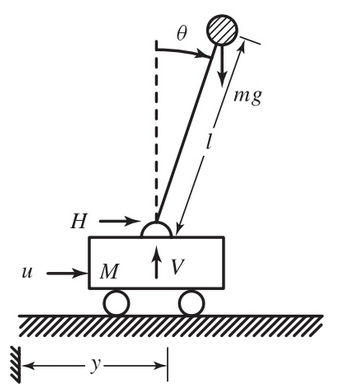
\includegraphics{./Figures/InvertedPendulum.png}
\caption{Inverted Pendulum}
\end{figure}

In this work, we will look at the properties of the system and check to
see if the system can be made controllable by either using Kalman
decomposition or pole placement

\section{Literature Review}\label{literature-review}

The course textbook {[}1{]} describes the mathematics in deriving the
state space equations that represent the system. The equations for the
system are given by: 
\[
\begin{bmatrix}
    \dot{x_1}(t)\\
    \dot{x_2}(t)\\
    \dot{x_3}(t)\\
    \dot{x_4}(t)\\
\end{bmatrix}=\begin{bmatrix}
    0 & 1 & 0 & 0 \\
    0 & 0 & \frac{-mg}{M} & 0 \\
    0 & 0 & 0 & 1 \\
    0 & 0 & \frac{(M+m)g}{Ml} & 0
    \end{bmatrix}\begin{bmatrix}
    x_1 \\
    x_2 \\
    x_3 \\
    x_4 \\
    \end{bmatrix} + \begin{bmatrix}
    0 \\ \frac{1}{M} \\ 0 \\ \frac{-1}{Ml}
    \end{bmatrix} u(t) 
 \]\[   \\
    y(t) = \begin{bmatrix}
    1 & 0 & 0 & 0
    \end{bmatrix}\mathbf{x}(t)
\]

where $ x_1(t) = y(t), x_2(t)=\dot{y}(t),x_3(t) =\theta(t),
\mathrm{and\ } x_4(t)=\dot{\theta}(t)$. As the goal of the system is
to maintain the attached mass in an upright postion, these equations are
only valid for \(\theta \rightarrow 0\). Furthermore, the output is only
set to the distance, \(y\), the cart needs to move from the starting
point.

A more realistic model is given in {[}2{]}. This model accounts for
friction between the cart wheels and the ground.

\[
\begin{bmatrix}
    \dot{x_1}(t)\\
    \dot{x_2}(t)\\
    \dot{x_3}(t)\\
    \dot{x_4}(t)\\
\end{bmatrix} = \begin{bmatrix}
    0 & 1 & 0 & 0 \\
    0 & \frac{-(I+ml^2)\mu}{I(M+m)+Mml^2} & \frac{m^2gl^2}{I(M+m)+Mml^2} &  0\\
    0 &      0      &        0    &       1\\
    0 &  \frac{-(ml\mu)}{I(M+m)+Mml^2}  &     \frac{mgl(M+m)}{I(M+m)+Mml^2} &  0 
\end{bmatrix}\begin{bmatrix}
    x_1 \\
    x_2 \\
    x_3 \\
    x_4 \\
    \end{bmatrix}+ \begin{bmatrix}
    0 \\ \frac{I+ml^2}{I(M+m)+Mml^2} \\ 0 \\ \frac{ml}{I(M+m)+Mml^2}
    \end{bmatrix} u(t) 
    \]\[
    y(t) = \begin{bmatrix}
    1 & 0 & 0 & 0\\
    0 & 0 & 1 & 0
    \end{bmatrix}\mathbf{x}(t)
\]
where, $I$ is the moment of inertia of the pendulum and $\mu$ is
the coefficient of friction between the ground and the cart's wheels.

For analysis, the first model is chosen for its simplicity

\section{Code and system}\label{code-and-system}

\subsection{Part I}\label{part-i}

\textbf{\emph{Set the Parameters to ensure the system is controllable
and observable. Prove the system is controllable and observable for the
chosen paparmeters.}}

    \begin{tcolorbox}[breakable, size=fbox, boxrule=1pt, pad at break*=1mm,colback=cellbackground, colframe=cellborder]
\prompt{In}{incolor}{1}{\boxspacing}
\begin{Verbatim}[commandchars=\\\{\}]
\PY{k+kn}{from} \PY{n+nn}{control} \PY{k+kn}{import} \PY{o}{*}
\PY{k+kn}{import} \PY{n+nn}{numpy} \PY{k}{as} \PY{n+nn}{np}
\PY{c+c1}{\PYZsh{}\PYZpc{}matplotlib}
\PY{k+kn}{import} \PY{n+nn}{matplotlib}\PY{n+nn}{.}\PY{n+nn}{pyplot} \PY{k}{as} \PY{n+nn}{plt}
\PY{k+kn}{from} \PY{n+nn}{matplotlib} \PY{k+kn}{import} \PY{n}{cm}
\PY{k+kn}{import} \PY{n+nn}{sympy} \PY{k}{as} \PY{n+nn}{sym}
\PY{k+kn}{from} \PY{n+nn}{IPython}\PY{n+nn}{.}\PY{n+nn}{display} \PY{k+kn}{import} \PY{n}{display}\PY{p}{,} \PY{n}{Markdown}
\PY{k+kn}{from} \PY{n+nn}{matplotlib}\PY{n+nn}{.}\PY{n+nn}{ticker} \PY{k+kn}{import} \PY{n}{LinearLocator}

\PY{k+kn}{from} \PY{n+nn}{control}\PY{n+nn}{.}\PY{n+nn}{matlab} \PY{k+kn}{import} \PY{o}{*}
\PY{n}{plt}\PY{o}{.}\PY{n}{rcParams}\PY{p}{[}\PY{l+s+s1}{\PYZsq{}}\PY{l+s+s1}{figure.figsize}\PY{l+s+s1}{\PYZsq{}}\PY{p}{]} \PY{o}{=} \PY{p}{[}\PY{l+m+mi}{10}\PY{p}{,} \PY{l+m+mi}{10}\PY{p}{]}
\end{Verbatim}
\end{tcolorbox}

    Set parameters for the inverted pendulum: Let 
\[
	g = 9.8 \mathrm{\ m/s^2} \]\[
	M = 2 \mathrm{\ kg} \]\[
	m = 1 \mathrm{\ kg} \]\[
    l = 0.5 \mathrm{\ m}
\]

    \begin{tcolorbox}[breakable, size=fbox, boxrule=1pt, pad at break*=1mm,colback=cellbackground, colframe=cellborder]
\prompt{In}{incolor}{34}{\boxspacing}
\begin{Verbatim}[commandchars=\\\{\}]
\PY{n}{m} \PY{o}{=} \PY{l+m+mi}{1} \PY{c+c1}{\PYZsh{} mass of the pendulum.}
\PY{n}{M} \PY{o}{=} \PY{l+m+mi}{2} \PY{c+c1}{\PYZsh{} mass of the cart.}
\PY{n}{g} \PY{o}{=} \PY{l+m+mf}{9.81} \PY{c+c1}{\PYZsh{} gravity.}
\PY{n}{l} \PY{o}{=} \PY{l+m+mf}{0.5} \PY{c+c1}{\PYZsh{} length of the pendulum.}

\PY{n}{A} \PY{o}{=} \PY{n}{np}\PY{o}{.}\PY{n}{array}\PY{p}{(}\PY{p}{[}\PY{p}{[}\PY{l+m+mi}{0}\PY{p}{,}\PY{l+m+mi}{1}\PY{p}{,}\PY{l+m+mi}{0}\PY{p}{,}\PY{l+m+mi}{0}\PY{p}{]}\PY{p}{,}\PY{p}{[}\PY{l+m+mi}{0}\PY{p}{,}\PY{l+m+mi}{0}\PY{p}{,}\PY{o}{\PYZhy{}}\PY{p}{(}\PY{n}{m}\PY{o}{*}\PY{n}{g}\PY{p}{)}\PY{o}{/}\PY{n}{M}\PY{p}{,}\PY{l+m+mi}{0}\PY{p}{]}\PY{p}{,}\PY{p}{[}\PY{l+m+mi}{0}\PY{p}{,}\PY{l+m+mi}{0}\PY{p}{,}\PY{l+m+mi}{0}\PY{p}{,}\PY{l+m+mi}{1}\PY{p}{]}\PY{p}{,}\PY{p}{[}\PY{l+m+mi}{0}\PY{p}{,}\PY{l+m+mi}{0}\PY{p}{,}\PY{p}{(}\PY{n}{M}\PY{o}{+}\PY{n}{m}\PY{p}{)}\PY{o}{*}\PY{n}{g}\PY{o}{/}\PY{p}{(}\PY{n}{M}\PY{o}{*}\PY{n}{l}\PY{p}{)}\PY{p}{,}\PY{l+m+mi}{0}\PY{p}{]}\PY{p}{]}\PY{p}{)} \PY{c+c1}{\PYZsh{}A is a system matrix.}
\PY{n}{B} \PY{o}{=} \PY{n}{np}\PY{o}{.}\PY{n}{array}\PY{p}{(}\PY{p}{[}\PY{p}{[}\PY{l+m+mi}{0}\PY{p}{]}\PY{p}{,}\PY{p}{[}\PY{l+m+mi}{1}\PY{o}{/}\PY{n}{M}\PY{p}{]}\PY{p}{,}\PY{p}{[}\PY{l+m+mi}{0}\PY{p}{]}\PY{p}{,}\PY{p}{[}\PY{o}{\PYZhy{}}\PY{l+m+mi}{1}\PY{o}{/}\PY{p}{(}\PY{n}{M}\PY{o}{*}\PY{n}{l}\PY{p}{)}\PY{p}{]}\PY{p}{]}\PY{p}{)} \PY{c+c1}{\PYZsh{}B is an input matrix.}
\PY{n}{C} \PY{o}{=} \PY{n}{np}\PY{o}{.}\PY{n}{array}\PY{p}{(}\PY{p}{[}\PY{l+m+mi}{1}\PY{p}{,}\PY{l+m+mi}{0}\PY{p}{,}\PY{l+m+mi}{0}\PY{p}{,}\PY{l+m+mi}{0}\PY{p}{]}\PY{p}{)} \PY{c+c1}{\PYZsh{}C is an Output matrix.}
\PY{n}{D} \PY{o}{=} \PY{l+m+mi}{0} \PY{c+c1}{\PYZsh{}D is a Transmission matrix}
\PY{n}{B}
\end{Verbatim}
\end{tcolorbox}

            \begin{tcolorbox}[breakable, size=fbox, boxrule=.5pt, pad at break*=1mm, opacityfill=0]
\prompt{Out}{outcolor}{34}{\boxspacing}
\begin{Verbatim}[commandchars=\\\{\}]
array([[ 0. ],
       [ 0.5],
       [ 0. ],
       [-1. ]])
\end{Verbatim}
\end{tcolorbox}
        
\subsubsection{Check the Controllabilty:}\label{check-the-controllabilty}

    \begin{tcolorbox}[breakable, size=fbox, boxrule=1pt, pad at break*=1mm,colback=cellbackground, colframe=cellborder]
\prompt{In}{incolor}{3}{\boxspacing}
\begin{Verbatim}[commandchars=\\\{\}]
\PY{n}{Co} \PY{o}{=} \PY{n}{ctrb}\PY{p}{(}\PY{n}{A}\PY{p}{,}\PY{n}{B}\PY{p}{)}                          \PY{c+c1}{\PYZsh{} Get the controlabillity matrix}
\PY{n}{rows}\PY{p}{,}\PY{n}{columns} \PY{o}{=} \PY{n}{np}\PY{o}{.}\PY{n}{shape}\PY{p}{(}\PY{n}{Co}\PY{p}{)}
\PY{n}{R1} \PY{o}{=} \PY{n}{np}\PY{o}{.}\PY{n}{linalg}\PY{o}{.}\PY{n}{matrix\PYZus{}rank}\PY{p}{(}\PY{n}{Co}\PY{p}{)}          \PY{c+c1}{\PYZsh{} Get the rank of the controllability matrix}
\PY{k}{if} \PY{n}{R1} \PY{o}{==} \PY{n}{rows} \PY{p}{:}                         \PY{c+c1}{\PYZsh{} Check if matrix has full row rank }
    \PY{n+nb}{print}\PY{p}{(}\PY{l+s+s2}{\PYZdq{}}\PY{l+s+s2}{System is Controllable.}\PY{l+s+s2}{\PYZdq{}}\PY{p}{)}
    \PY{n}{de1} \PY{o}{=} \PY{n}{np}\PY{o}{.}\PY{n}{linalg}\PY{o}{.}\PY{n}{det}\PY{p}{(}\PY{n}{Co}\PY{p}{)}
    \PY{n+nb}{print}\PY{p}{(}\PY{n}{de1}\PY{p}{)} 
\PY{k}{else}\PY{p}{:}
    \PY{n+nb}{print}\PY{p}{(}\PY{l+s+s2}{\PYZdq{}}\PY{l+s+s2}{System is not Controllable}\PY{l+s+s2}{\PYZdq{}}\PY{p}{)}
\end{Verbatim}
\end{tcolorbox}

    \begin{Verbatim}[commandchars=\\\{\}]
System is Controlable.
96.2361
    \end{Verbatim}

    As can be seen, the system is controllabe since the controllability
matrix \(\mathcal{C}_o\) has full row rank. Further, the determinant of
matrix \(\mathcal{C}_o\) is non zero.

\subsubsection{Check the Observability:}\label{check-the-observability}

    \begin{tcolorbox}[breakable, size=fbox, boxrule=1pt, pad at break*=1mm,colback=cellbackground, colframe=cellborder]
\prompt{In}{incolor}{4}{\boxspacing}
\begin{Verbatim}[commandchars=\\\{\}]
\PY{n}{Obs} \PY{o}{=} \PY{n}{obsv}\PY{p}{(}\PY{n}{A}\PY{p}{,}\PY{n}{C}\PY{p}{)}                    \PY{c+c1}{\PYZsh{} Get the observability matrix}
\PY{n}{rows}\PY{p}{,}\PY{n}{columns} \PY{o}{=} \PY{n}{np}\PY{o}{.}\PY{n}{shape}\PY{p}{(}\PY{n}{Obs}\PY{p}{)}
\PY{n}{R2}\PY{o}{=}\PY{n}{np}\PY{o}{.}\PY{n}{linalg}\PY{o}{.}\PY{n}{matrix\PYZus{}rank}\PY{p}{(}\PY{n}{Obs}\PY{p}{)}      \PY{c+c1}{\PYZsh{} Get the rank of the observability matrix}
\PY{k}{if} \PY{n}{R2} \PY{o}{==} \PY{n}{rows}\PY{p}{:}                     \PY{c+c1}{\PYZsh{} Check if matrix has full row rank}
    \PY{n+nb}{print}\PY{p}{(}\PY{l+s+s2}{\PYZdq{}}\PY{l+s+s2}{System is observable.}\PY{l+s+s2}{\PYZdq{}}\PY{p}{)}
    \PY{n}{de2} \PY{o}{=} \PY{n}{np}\PY{o}{.}\PY{n}{linalg}\PY{o}{.}\PY{n}{det}\PY{p}{(}\PY{n}{Obs}\PY{p}{)}
    \PY{n+nb}{print}\PY{p}{(}\PY{n}{de2}\PY{p}{)} 
\PY{k}{else}\PY{p}{:}
    \PY{n+nb}{print}\PY{p}{(}\PY{l+s+s2}{\PYZdq{}}\PY{l+s+s2}{System is not observable}\PY{l+s+s2}{\PYZdq{}}\PY{p}{)}
\end{Verbatim}
\end{tcolorbox}

    \begin{Verbatim}[commandchars=\\\{\}]
System is observable.
24.059025000000005
    \end{Verbatim}

    The system is observable as well. The observability matrix
\(\mathcal{O}\) is also full rank. Further, the determinant of matrix
\(\mathcal{O}\) is non zero.

\subsubsection{Regions of Control}\label{regions-of-control}

The matrix may be controllable and observable for the given values. But
to check for values that the system might not be controllable or
observable, we can solve for the determinant algebraicly. If the
determinant of a matrix is non zero, it can be shown that the rank of
the matrix is less than full rank.

    \begin{tcolorbox}[breakable, size=fbox, boxrule=1pt, pad at break*=1mm,colback=cellbackground, colframe=cellborder]
\prompt{In}{incolor}{5}{\boxspacing}
\begin{Verbatim}[commandchars=\\\{\}]
\PY{n}{M}\PY{p}{,}\PY{n}{m}\PY{p}{,}\PY{n}{l} \PY{o}{=} \PY{n}{sym}\PY{o}{.}\PY{n}{symbols}\PY{p}{(}\PY{l+s+s1}{\PYZsq{}}\PY{l+s+s1}{M m l}\PY{l+s+s1}{\PYZsq{}}\PY{p}{)}

\PY{n}{A} \PY{o}{=} \PY{n}{sym}\PY{o}{.}\PY{n}{Matrix}\PY{p}{(}\PY{p}{[}\PY{p}{[}\PY{l+m+mi}{0}\PY{p}{,}\PY{l+m+mi}{1}\PY{p}{,}\PY{l+m+mi}{0}\PY{p}{,}\PY{l+m+mi}{0}\PY{p}{]}\PY{p}{,}\PY{p}{[}\PY{l+m+mi}{0}\PY{p}{,}\PY{l+m+mi}{0}\PY{p}{,}\PY{o}{\PYZhy{}}\PY{p}{(}\PY{n}{m}\PY{o}{*}\PY{n}{g}\PY{p}{)}\PY{o}{/}\PY{n}{M}\PY{p}{,}\PY{l+m+mi}{0}\PY{p}{]}\PY{p}{,}\PY{p}{[}\PY{l+m+mi}{0}\PY{p}{,}\PY{l+m+mi}{0}\PY{p}{,}\PY{l+m+mi}{0}\PY{p}{,}\PY{l+m+mi}{1}\PY{p}{]}\PY{p}{,}\PY{p}{[}\PY{l+m+mi}{0}\PY{p}{,}\PY{l+m+mi}{0}\PY{p}{,}\PY{p}{(}\PY{n}{M}\PY{o}{+}\PY{n}{m}\PY{p}{)}\PY{o}{*}\PY{n}{g}\PY{o}{/}\PY{p}{(}\PY{n}{M}\PY{o}{*}\PY{n}{l}\PY{p}{)}\PY{p}{,}\PY{l+m+mi}{0}\PY{p}{]}\PY{p}{]}\PY{p}{)} \PY{c+c1}{\PYZsh{}A is a system matrix.}
\PY{n}{B} \PY{o}{=} \PY{n}{sym}\PY{o}{.}\PY{n}{Matrix}\PY{p}{(}\PY{p}{[}\PY{l+m+mi}{0}\PY{p}{,}\PY{l+m+mi}{1}\PY{o}{/}\PY{n}{M}\PY{p}{,}\PY{l+m+mi}{0}\PY{p}{,}\PY{o}{\PYZhy{}}\PY{l+m+mi}{1}\PY{o}{/}\PY{p}{(}\PY{n}{M}\PY{o}{*}\PY{n}{l}\PY{p}{)}\PY{p}{]}\PY{p}{)} \PY{c+c1}{\PYZsh{}B is an input matrix.}
\PY{n}{C} \PY{o}{=} \PY{n}{sym}\PY{o}{.}\PY{n}{Matrix}\PY{p}{(}\PY{p}{[}\PY{l+m+mi}{1}\PY{p}{,}\PY{l+m+mi}{0}\PY{p}{,}\PY{l+m+mi}{0}\PY{p}{,}\PY{l+m+mi}{0}\PY{p}{]}\PY{p}{)}
\PY{n}{C} \PY{o}{=} \PY{n}{C}\PY{o}{.}\PY{n}{T}
\end{Verbatim}
\end{tcolorbox}

    Since we're doing this algebraicly, we need to manually make the
controllability and observability matrix. and find the determinant

    \begin{tcolorbox}[breakable, size=fbox, boxrule=1pt, pad at break*=1mm,colback=cellbackground, colframe=cellborder]
\prompt{In}{incolor}{6}{\boxspacing}
\begin{Verbatim}[commandchars=\\\{\}]
\PY{n}{Ctrb} \PY{o}{=} \PY{n}{B}
\PY{n}{Ctrb} \PY{o}{=} \PY{n}{Ctrb}\PY{o}{.}\PY{n}{col\PYZus{}insert}\PY{p}{(}\PY{l+m+mi}{1}\PY{p}{,}\PY{n}{A}\PY{o}{*}\PY{n}{B}\PY{p}{)}
\PY{n}{Ctrb} \PY{o}{=} \PY{n}{Ctrb}\PY{o}{.}\PY{n}{col\PYZus{}insert}\PY{p}{(}\PY{l+m+mi}{2}\PY{p}{,}\PY{n}{A}\PY{o}{*}\PY{n}{A}\PY{o}{*}\PY{n}{B}\PY{p}{)}
\PY{n}{Ctrb} \PY{o}{=} \PY{n}{Ctrb}\PY{o}{.}\PY{n}{col\PYZus{}insert}\PY{p}{(}\PY{l+m+mi}{3}\PY{p}{,}\PY{n}{A}\PY{o}{*}\PY{n}{A}\PY{o}{*}\PY{n}{A}\PY{o}{*}\PY{n}{B}\PY{p}{)}
\PY{n}{Ctrb\PYZus{}det} \PY{o}{=} \PY{n}{Ctrb}\PY{o}{.}\PY{n}{det}\PY{p}{(}\PY{p}{)}
\PY{n}{Ctrb\PYZus{}det}
\end{Verbatim}
\end{tcolorbox}
 
            
\prompt{Out}{outcolor}{6}{}
    
    $\displaystyle \frac{96.2361}{M^{4} l^{4}}$

    

    This shows that the system is un-controllable for values of
\(M \ \mathrm{and}\  l \rightarrow \infty\)

    \begin{tcolorbox}[breakable, size=fbox, boxrule=1pt, pad at break*=1mm,colback=cellbackground, colframe=cellborder]
\prompt{In}{incolor}{7}{\boxspacing}
\begin{Verbatim}[commandchars=\\\{\}]
\PY{n}{Obs} \PY{o}{=} \PY{n}{C}
\PY{n}{Obs} \PY{o}{=} \PY{n}{Obs}\PY{o}{.}\PY{n}{row\PYZus{}insert}\PY{p}{(}\PY{l+m+mi}{1}\PY{p}{,}\PY{n}{C}\PY{o}{*}\PY{n}{A}\PY{p}{)}
\PY{n}{Obs} \PY{o}{=} \PY{n}{Obs}\PY{o}{.}\PY{n}{row\PYZus{}insert}\PY{p}{(}\PY{l+m+mi}{2}\PY{p}{,}\PY{n}{C}\PY{o}{*}\PY{n}{A}\PY{o}{*}\PY{n}{A}\PY{p}{)}
\PY{n}{Obs} \PY{o}{=} \PY{n}{Obs}\PY{o}{.}\PY{n}{row\PYZus{}insert}\PY{p}{(}\PY{l+m+mi}{3}\PY{p}{,}\PY{n}{C}\PY{o}{*}\PY{n}{A}\PY{o}{*}\PY{n}{A}\PY{o}{*}\PY{n}{A}\PY{p}{)}
\PY{n}{Obs\PYZus{}det} \PY{o}{=} \PY{n}{Obs}\PY{o}{.}\PY{n}{det}\PY{p}{(}\PY{p}{)}
\PY{n}{Obs\PYZus{}det}
\end{Verbatim}
\end{tcolorbox}
 
            
\prompt{Out}{outcolor}{7}{}
    
    $\displaystyle \frac{96.2361 m^{2}}{M^{2}}$

    

    This shows that the system is un-observable for values of
\(M \rightarrow \infty\) or \(m = 0\)

\subsection{Part II}\label{part-ii}

\textbf{\emph{Set the parameters to create an ``uncontrollable'' form
and use Kalman Decomposition to obtain the controllable form.}}

For this part, the first step was to figure out what values of
parameters would make the system uncontrollable. If the rank of the
controllability matrix was forced to be made less than the full rank,
the system would become uncontrollable. The following code calculates
the controllability matrix of the given system.

    \begin{tcolorbox}[breakable, size=fbox, boxrule=1pt, pad at break*=1mm,colback=cellbackground, colframe=cellborder]
\prompt{In}{incolor}{8}{\boxspacing}
\begin{Verbatim}[commandchars=\\\{\}]
\PY{c+c1}{\PYZsh{} This is for nice looking latex output}
\PY{n}{sym}\PY{o}{.}\PY{n}{init\PYZus{}printing}\PY{p}{(}\PY{p}{)}

\PY{c+c1}{\PYZsh{} Defining our system matrices}
\PY{n}{m}\PY{p}{,} \PY{n}{M}\PY{p}{,} \PY{n}{l}\PY{p}{,} \PY{n}{g} \PY{o}{=} \PY{n}{sym}\PY{o}{.}\PY{n}{symbols}\PY{p}{(}\PY{l+s+s1}{\PYZsq{}}\PY{l+s+s1}{m M l g}\PY{l+s+s1}{\PYZsq{}}\PY{p}{)}

\PY{n}{A} \PY{o}{=} \PY{n}{sym}\PY{o}{.}\PY{n}{Matrix}\PY{p}{(}\PY{p}{[}\PY{p}{[}\PY{l+m+mi}{0}\PY{p}{,} \PY{l+m+mi}{1}\PY{p}{,} \PY{l+m+mi}{0}\PY{p}{,} \PY{l+m+mi}{0}\PY{p}{]}\PY{p}{,}
               \PY{p}{[}\PY{l+m+mi}{0}\PY{p}{,} \PY{l+m+mi}{0}\PY{p}{,} \PY{o}{\PYZhy{}}\PY{n}{m}\PY{o}{*}\PY{n}{g}\PY{o}{/}\PY{n}{M}\PY{p}{,} \PY{l+m+mi}{0}\PY{p}{]}\PY{p}{,}
               \PY{p}{[}\PY{l+m+mi}{0}\PY{p}{,} \PY{l+m+mi}{0}\PY{p}{,} \PY{l+m+mi}{0}\PY{p}{,} \PY{l+m+mi}{1}\PY{p}{]}\PY{p}{,}
               \PY{p}{[}\PY{l+m+mi}{0}\PY{p}{,} \PY{l+m+mi}{0}\PY{p}{,} \PY{p}{(}\PY{n}{M}\PY{o}{+}\PY{n}{m}\PY{p}{)}\PY{o}{*}\PY{n}{g}\PY{o}{/}\PY{p}{(}\PY{n}{M}\PY{o}{*}\PY{n}{l}\PY{p}{)}\PY{p}{,} \PY{l+m+mi}{0}\PY{p}{]}\PY{p}{]}\PY{p}{)}

\PY{n}{B} \PY{o}{=} \PY{n}{sym}\PY{o}{.}\PY{n}{Matrix}\PY{p}{(}\PY{p}{[}\PY{p}{[}\PY{l+m+mi}{0}\PY{p}{]}\PY{p}{,}
               \PY{p}{[}\PY{l+m+mi}{1}\PY{o}{/}\PY{n}{M}\PY{p}{]}\PY{p}{,}
               \PY{p}{[}\PY{l+m+mi}{0}\PY{p}{]}\PY{p}{,}
               \PY{p}{[}\PY{o}{\PYZhy{}}\PY{l+m+mi}{1}\PY{o}{/}\PY{p}{(}\PY{n}{M}\PY{o}{*}\PY{n}{l}\PY{p}{)}\PY{p}{]}\PY{p}{]}\PY{p}{)}

\PY{n}{C} \PY{o}{=} \PY{n}{sym}\PY{o}{.}\PY{n}{Matrix}\PY{p}{(}\PY{p}{[}\PY{p}{[}\PY{l+m+mi}{1}\PY{p}{,} \PY{l+m+mi}{0}\PY{p}{,} \PY{l+m+mi}{0}\PY{p}{,} \PY{l+m+mi}{0}\PY{p}{]}\PY{p}{]}\PY{p}{)}

\PY{c+c1}{\PYZsh{} This function returns True if the parameter num is a float. False, otherwise.}
\PY{k}{def} \PY{n+nf}{isfloat}\PY{p}{(}\PY{n}{num}\PY{p}{)}\PY{p}{:}
    \PY{k}{try}\PY{p}{:}
        \PY{n+nb}{float}\PY{p}{(}\PY{n}{num}\PY{p}{)}
        \PY{k}{return} \PY{k+kc}{True}
    \PY{k}{except} \PY{n+ne}{ValueError}\PY{p}{:}
        \PY{k}{return} \PY{k+kc}{False}

\PY{c+c1}{\PYZsh{} This function returns whether or not a particular matrix is controllable. The matrices must only be symbolic matrices. }
\PY{c+c1}{\PYZsh{} It also returns the controllability matrix. }
\PY{k}{def} \PY{n+nf}{controllable\PYZus{}sym}\PY{p}{(}\PY{n}{A}\PY{p}{,} \PY{n}{B}\PY{p}{,} \PY{n}{dim}\PY{o}{=}\PY{l+m+mi}{4}\PY{p}{)}\PY{p}{:}
    \PY{n}{cols} \PY{o}{=} \PY{n}{B}
    
    \PY{k}{for} \PY{n}{i} \PY{o+ow}{in} \PY{n+nb}{range}\PY{p}{(}\PY{l+m+mi}{1}\PY{p}{,} \PY{n}{dim}\PY{p}{)}\PY{p}{:}
        \PY{n}{col} \PY{o}{=} \PY{n}{sym}\PY{o}{.}\PY{n}{Matrix}\PY{p}{(}\PY{p}{[}\PY{p}{[}\PY{p}{(}\PY{n}{A}\PY{o}{*}\PY{o}{*}\PY{n}{i}\PY{p}{)}\PY{o}{*}\PY{n}{B}\PY{p}{]}\PY{p}{]}\PY{p}{)}
        \PY{n}{cols} \PY{o}{=} \PY{n}{cols}\PY{o}{.}\PY{n}{col\PYZus{}insert}\PY{p}{(}\PY{n}{i}\PY{p}{,} \PY{n}{col}\PY{p}{)}
    
    \PY{k}{if}\PY{p}{(}\PY{n}{cols}\PY{o}{.}\PY{n}{rank}\PY{p}{(}\PY{p}{)} \PY{o}{==} \PY{n}{dim}\PY{p}{)}\PY{p}{:}
        \PY{k}{return} \PY{k+kc}{True}\PY{p}{,} \PY{n}{cols}
    \PY{k}{else}\PY{p}{:}
        \PY{k}{return} \PY{k+kc}{False}\PY{p}{,} \PY{n}{cols}
    

\PY{n}{controllable}\PY{p}{,} \PY{n}{cont\PYZus{}matrix} \PY{o}{=} \PY{n}{controllable\PYZus{}sym}\PY{p}{(}\PY{n}{A}\PY{p}{,} \PY{n}{B}\PY{p}{)}

\PY{c+c1}{\PYZsh{} displaying the controllability Matrix}
\PY{n}{cont\PYZus{}matrix}
\end{Verbatim}
\end{tcolorbox}
 
            
\prompt{Out}{outcolor}{8}{}
    
    $\displaystyle \left[\begin{matrix}0 & \frac{1}{M} & 0 & \frac{g m}{M^{2} l}\\\frac{1}{M} & 0 & \frac{g m}{M^{2} l} & 0\\0 & - \frac{1}{M l} & 0 & - \frac{g \left(M + m\right)}{M^{2} l^{2}}\\- \frac{1}{M l} & 0 & - \frac{g \left(M + m\right)}{M^{2} l^{2}} & 0\end{matrix}\right]$

    

    The goal now is to make column 1 equal to column 3. (1 indexed)

We can to by the following 2 rules:

\[ 
 m >>> M \]\[
 M = \frac{gm}{l}
\]

In the following code, we will define the variables according to the
above rules and verify that this new system is, in fact, uncontrollable.

    \begin{tcolorbox}[breakable, size=fbox, boxrule=1pt, pad at break*=1mm,colback=cellbackground, colframe=cellborder]
\prompt{In}{incolor}{9}{\boxspacing}
\begin{Verbatim}[commandchars=\\\{\}]
\PY{c+c1}{\PYZsh{} This function checks to see if a numerical matrix consisting of floats is controllable. }
\PY{c+c1}{\PYZsh{} It returns the boolean value along with the controllability matrix. }
\PY{k}{def} \PY{n+nf}{controllable}\PY{p}{(}\PY{n}{A}\PY{p}{,} \PY{n}{B}\PY{p}{,} \PY{n}{dim}\PY{o}{=}\PY{l+m+mi}{4}\PY{p}{)}\PY{p}{:}
    \PY{n}{cols} \PY{o}{=} \PY{n}{B}
    
    \PY{k}{for} \PY{n}{i} \PY{o+ow}{in} \PY{n+nb}{range}\PY{p}{(}\PY{l+m+mi}{1}\PY{p}{,} \PY{n}{dim}\PY{p}{)}\PY{p}{:}
        \PY{n}{col} \PY{o}{=} \PY{n}{sym}\PY{o}{.}\PY{n}{Matrix}\PY{p}{(}\PY{p}{[}\PY{p}{[}\PY{p}{(}\PY{n}{A}\PY{o}{*}\PY{o}{*}\PY{n}{i}\PY{p}{)}\PY{o}{*}\PY{n}{B}\PY{p}{]}\PY{p}{]}\PY{p}{)}
        \PY{n}{cols} \PY{o}{=} \PY{n}{cols}\PY{o}{.}\PY{n}{col\PYZus{}insert}\PY{p}{(}\PY{n}{i}\PY{p}{,} \PY{n}{col}\PY{p}{)}
    
    \PY{n}{r}\PY{p}{,} \PY{n}{c} \PY{o}{=} \PY{n}{sym}\PY{o}{.}\PY{n}{shape}\PY{p}{(}\PY{n}{cols}\PY{p}{)}
    
    \PY{k}{for} \PY{n}{i} \PY{o+ow}{in} \PY{n+nb}{range}\PY{p}{(}\PY{n}{r}\PY{o}{*}\PY{n}{c}\PY{p}{)}\PY{p}{:}
        \PY{k}{if}\PY{p}{(}\PY{n}{isfloat}\PY{p}{(}\PY{n}{cols}\PY{p}{[}\PY{n}{i}\PY{p}{]}\PY{p}{)}\PY{p}{)}\PY{p}{:}
            \PY{n}{cols}\PY{p}{[}\PY{n}{i}\PY{p}{]} \PY{o}{=} \PY{n+nb}{round}\PY{p}{(}\PY{n}{cols}\PY{p}{[}\PY{n}{i}\PY{p}{]}\PY{p}{,} \PY{l+m+mi}{2}\PY{p}{)}
    
    \PY{k}{if}\PY{p}{(}\PY{n}{cols}\PY{o}{.}\PY{n}{rank}\PY{p}{(}\PY{p}{)} \PY{o}{==} \PY{n}{dim}\PY{p}{)}\PY{p}{:}
        \PY{k}{return} \PY{k+kc}{True}\PY{p}{,} \PY{n}{cols}
    \PY{k}{else}\PY{p}{:}
        \PY{k}{return} \PY{k+kc}{False}\PY{p}{,} \PY{n}{cols}

\PY{n}{calc\PYZus{}m} \PY{o}{=} \PY{l+m+mi}{10000}
\PY{n}{calc\PYZus{}g} \PY{o}{=} \PY{l+m+mf}{9.8}
\PY{n}{calc\PYZus{}l} \PY{o}{=} \PY{l+m+mi}{9900}
\PY{n}{calc\PYZus{}M} \PY{o}{=} \PY{p}{(}\PY{n}{calc\PYZus{}g}\PY{o}{*}\PY{n}{calc\PYZus{}m}\PY{p}{)}\PY{o}{/}\PY{p}{(}\PY{n}{calc\PYZus{}l}\PY{p}{)}


\PY{n}{new\PYZus{}A} \PY{o}{=} \PY{n}{A}\PY{o}{.}\PY{n}{evalf}\PY{p}{(}\PY{n}{subs}\PY{o}{=}\PY{p}{\PYZob{}}\PY{n}{m}\PY{p}{:}\PY{n}{calc\PYZus{}m}\PY{p}{,} \PY{n}{M}\PY{p}{:}\PY{n}{calc\PYZus{}M}\PY{p}{,} \PY{n}{l}\PY{p}{:}\PY{n}{calc\PYZus{}l} \PY{p}{,} \PY{n}{g}\PY{p}{:}\PY{n}{calc\PYZus{}g}\PY{p}{\PYZcb{}}\PY{p}{)}
\PY{n}{new\PYZus{}B} \PY{o}{=} \PY{n}{B}\PY{o}{.}\PY{n}{evalf}\PY{p}{(}\PY{n}{subs}\PY{o}{=}\PY{p}{\PYZob{}}\PY{n}{m}\PY{p}{:}\PY{n}{calc\PYZus{}m}\PY{p}{,} \PY{n}{M}\PY{p}{:}\PY{n}{calc\PYZus{}M}\PY{p}{,} \PY{n}{l}\PY{p}{:}\PY{n}{calc\PYZus{}l} \PY{p}{,} \PY{n}{g}\PY{p}{:}\PY{n}{calc\PYZus{}g}\PY{p}{\PYZcb{}}\PY{p}{)}
\PY{n}{new\PYZus{}C} \PY{o}{=} \PY{n}{C}\PY{o}{.}\PY{n}{evalf}\PY{p}{(}\PY{n}{subs}\PY{o}{=}\PY{p}{\PYZob{}}\PY{n}{m}\PY{p}{:}\PY{n}{calc\PYZus{}m}\PY{p}{,} \PY{n}{M}\PY{p}{:}\PY{n}{calc\PYZus{}M}\PY{p}{,} \PY{n}{l}\PY{p}{:}\PY{n}{calc\PYZus{}l} \PY{p}{,} \PY{n}{g}\PY{p}{:}\PY{n}{calc\PYZus{}g}\PY{p}{\PYZcb{}}\PY{p}{)}

\PY{n}{new\PYZus{}controllable}\PY{p}{,} \PY{n}{new\PYZus{}cont\PYZus{}matrix} \PY{o}{=} \PY{n}{controllable}\PY{p}{(}\PY{n}{new\PYZus{}A}\PY{p}{,} \PY{n}{new\PYZus{}B}\PY{p}{)}

\PY{n+nb}{print}\PY{p}{(}\PY{l+s+s2}{\PYZdq{}}\PY{l+s+s2}{controllable?}\PY{l+s+s2}{\PYZdq{}}\PY{p}{,} \PY{n}{new\PYZus{}controllable}\PY{p}{)}

\PY{c+c1}{\PYZsh{} display the new controllability matrix }
\PY{n}{new\PYZus{}cont\PYZus{}matrix}
\end{Verbatim}
\end{tcolorbox}

    \begin{Verbatim}[commandchars=\\\{\}]
controllable? False
    \end{Verbatim}
 
            
\prompt{Out}{outcolor}{9}{}
    
    $\displaystyle \left[\begin{matrix}0 & 0.1 & 0 & 0.1\\0.1 & 0 & 0.1 & 0\\0 & 0 & 0 & 0\\0 & 0 & 0 & 0\end{matrix}\right]$

    

    \begin{tcolorbox}[breakable, size=fbox, boxrule=1pt, pad at break*=1mm,colback=cellbackground, colframe=cellborder]
\prompt{In}{incolor}{10}{\boxspacing}
\begin{Verbatim}[commandchars=\\\{\}]
\PY{n+nb}{print}\PY{p}{(}\PY{l+s+s2}{\PYZdq{}}\PY{l+s+s2}{Rank of the above Controllable Matrix:}\PY{l+s+s2}{\PYZdq{}}\PY{p}{,} \PY{n}{new\PYZus{}cont\PYZus{}matrix}\PY{o}{.}\PY{n}{rank}\PY{p}{(}\PY{p}{)}\PY{p}{)}
\end{Verbatim}
\end{tcolorbox}

    \begin{Verbatim}[commandchars=\\\{\}]
Rank of the above Controllable Matrix: 2
    \end{Verbatim}

\subsubsection{Kalman Decomposition}\label{kalman-decomposition}

Since the rank of this new matrix is 2 (less than 4), the new system is
not controllable. We can make it controllable using the method of Kalman
Decomposition. Let's understand the Kalman Decomposition Process.

\begin{enumerate}
\def\labelenumi{\arabic{enumi}.}
\item
  We generate a matrix Q using the controllability matrix such that Q is
  inversible. Since the rank of our controllability matrix was 2, we
  will use 2 linearly independent columns of the controllability matrix
  as the first 2 columns of Q. We will then fill in the rest of Q such
  that Q is invertible. In our code, we will simply find the nullspace
  of the 2 vectors we get from the controllability matrix.

  \[Q = \begin{bmatrix} 0 & 0.1 & 0 & 0 \\ 0.1 & 0 & 0 & 0 \\ 0 & 0 & 1 & 0\\ 0 & 0 & 0 & 1 \end{bmatrix}\]
\item
  Find P

  \[ P = Q^{-1} \]
\item
  Find $ \bar{A} $ , $ \bar{B} $, $ \bar{C} $ with the
  following formulae:

  \[ \bar{A} = PAP^{-1} \] \[ \bar{B} = PB \] \[ \bar{C} = CP^{-1} \]
\item
  Finally, we pick the 2x2 top left of $ \bar{A} $ (2x2 because A is
  a square matrix and the rank of our original controllability matrix
  was 2) and name it $ A_c $. We pick 2x1 of the $ \bar{B} $ and
  name it $ B_c $. And we pick 1x2 of the $ \bar{C} $ and name it
  $ C_c $
\end{enumerate}

These new matrices that we found, $ A_c $, $ B_c $, $ C_c $,
make up the new representation of the system that is controllable. Now
that we've got the theory down, let's code it up and see the results.

\[ \dot{x} = A_c x(t) + B_c u(t) \] \[ y = C_c x(t) \]

    \begin{tcolorbox}[breakable, size=fbox, boxrule=1pt, pad at break*=1mm,colback=cellbackground, colframe=cellborder]
\prompt{In}{incolor}{11}{\boxspacing}
\begin{Verbatim}[commandchars=\\\{\}]
\PY{c+c1}{\PYZsh{} This function find the nullspace of the passed in matrix and adds the nullspace to the matrix. This new matrix is now invertible. }
\PY{k}{def} \PY{n+nf}{fill\PYZus{}square\PYZus{}with\PYZus{}identity}\PY{p}{(}\PY{n}{A}\PY{p}{)}\PY{p}{:}
    \PY{n}{row}\PY{p}{,} \PY{n}{col} \PY{o}{=} \PY{n}{sym}\PY{o}{.}\PY{n}{shape}\PY{p}{(}\PY{n}{A}\PY{p}{)}
    
    \PY{k}{if}\PY{p}{(}\PY{n}{row} \PY{o}{==} \PY{n}{col}\PY{p}{)}\PY{p}{:}
        \PY{k}{return} \PY{n}{A}
    
    \PY{k}{else}\PY{p}{:}
        \PY{k}{if}\PY{p}{(} \PY{n}{col} \PY{o}{\PYZlt{}} \PY{n}{row} \PY{p}{)}\PY{p}{:}
            \PY{n}{tempA} \PY{o}{=} \PY{n}{A}
            \PY{k}{for} \PY{n}{i}\PY{p}{,} \PY{n}{c} \PY{o+ow}{in} \PY{n+nb}{enumerate}\PY{p}{(}\PY{n}{A}\PY{o}{.}\PY{n}{T}\PY{o}{.}\PY{n}{nullspace}\PY{p}{(}\PY{p}{)}\PY{p}{)}\PY{p}{:}
                \PY{n}{A} \PY{o}{=} \PY{n}{A}\PY{o}{.}\PY{n}{col\PYZus{}insert}\PY{p}{(}\PY{n}{tempA}\PY{o}{.}\PY{n}{rank}\PY{p}{(}\PY{p}{)}\PY{o}{+}\PY{n}{i}\PY{p}{,} \PY{n}{c}\PY{p}{)}
            
            \PY{k}{return} \PY{n}{A}
                    
        \PY{k}{else}\PY{p}{:}
           \PY{n+nb}{print}\PY{p}{(}\PY{l+s+s2}{\PYZdq{}}\PY{l+s+s2}{something went wrong}\PY{l+s+s2}{\PYZdq{}}\PY{p}{)}
           \PY{k}{return} \PY{k+kc}{False}
        
    
\PY{c+c1}{\PYZsh{} This function performs the Kalman Decomposition using the passed in matrices. It returns the controllable matrices, namely Ac, Bc and Cc. }
\PY{k}{def} \PY{n+nf}{kalman\PYZus{}decomposition}\PY{p}{(}\PY{n}{A}\PY{p}{,} \PY{n}{B}\PY{p}{,} \PY{n}{controllability\PYZus{}matrix}\PY{p}{)}\PY{p}{:}
    
    \PY{n}{rank} \PY{o}{=} \PY{n}{controllability\PYZus{}matrix}\PY{o}{.}\PY{n}{rank}\PY{p}{(}\PY{p}{)}
    \PY{c+c1}{\PYZsh{} assuming that rank is atleast 1}
    \PY{n}{Q} \PY{o}{=} \PY{n}{controllability\PYZus{}matrix}\PY{o}{.}\PY{n}{col}\PY{p}{(}\PY{l+m+mi}{0}\PY{p}{)}
    
    \PY{k}{for} \PY{n}{i} \PY{o+ow}{in} \PY{n+nb}{range}\PY{p}{(}\PY{l+m+mi}{1}\PY{p}{,} \PY{n}{rank}\PY{p}{)}\PY{p}{:}
        \PY{n}{Q} \PY{o}{=} \PY{n}{Q}\PY{o}{.}\PY{n}{col\PYZus{}insert}\PY{p}{(}\PY{n}{i}\PY{p}{,} \PY{n}{controllability\PYZus{}matrix}\PY{o}{.}\PY{n}{col}\PY{p}{(}\PY{n}{i}\PY{p}{)}\PY{p}{)}
    
    \PY{n}{Q} \PY{o}{=} \PY{n}{fill\PYZus{}square\PYZus{}with\PYZus{}identity}\PY{p}{(}\PY{n}{Q}\PY{p}{)}
        
    \PY{k}{if}\PY{p}{(} \PY{o+ow}{not}\PY{p}{(}\PY{n}{Q}\PY{p}{)} \PY{p}{)}\PY{p}{:}
        \PY{k}{return} \PY{k+kc}{False}

    \PY{n}{P} \PY{o}{=} \PY{n}{Q}\PY{o}{.}\PY{n}{inv}\PY{p}{(}\PY{p}{)}
    \PY{n}{A\PYZus{}bar} \PY{o}{=} \PY{n}{P}\PY{o}{*}\PY{n}{A}\PY{o}{*}\PY{n}{P}\PY{o}{.}\PY{n}{inv}\PY{p}{(}\PY{p}{)}
    \PY{n}{B\PYZus{}bar} \PY{o}{=} \PY{n}{P}\PY{o}{*}\PY{n}{B}
    \PY{n}{C\PYZus{}bar} \PY{o}{=} \PY{n}{C}\PY{o}{*}\PY{n}{P}\PY{o}{.}\PY{n}{inv}\PY{p}{(}\PY{p}{)}
    
    \PY{n}{Ac} \PY{o}{=} \PY{n}{sym}\PY{o}{.}\PY{n}{Matrix}\PY{p}{(}\PY{p}{[}\PY{n}{A\PYZus{}bar}\PY{p}{[}\PY{p}{:}\PY{n}{rank}\PY{p}{,} \PY{p}{:}\PY{n}{rank}\PY{p}{]}\PY{p}{]}\PY{p}{)}
    \PY{n}{Bc} \PY{o}{=} \PY{n}{sym}\PY{o}{.}\PY{n}{Matrix}\PY{p}{(}\PY{p}{[}\PY{n}{B\PYZus{}bar}\PY{p}{[}\PY{p}{:}\PY{n}{rank}\PY{p}{]}\PY{p}{]}\PY{p}{)}\PY{o}{.}\PY{n}{T}
    \PY{n}{Cc} \PY{o}{=} \PY{n}{sym}\PY{o}{.}\PY{n}{Matrix}\PY{p}{(}\PY{p}{[}\PY{n}{C\PYZus{}bar}\PY{p}{[}\PY{p}{:}\PY{n}{rank}\PY{p}{]}\PY{p}{]}\PY{p}{)}
    
    \PY{k}{if}\PY{p}{(}\PY{o+ow}{not}\PY{p}{(}\PY{n}{controllable}\PY{p}{(}\PY{n}{Ac}\PY{p}{,} \PY{n}{Bc}\PY{p}{,} \PY{n}{rank}\PY{p}{)}\PY{p}{)}\PY{p}{)}\PY{p}{:}
        \PY{n+nb}{print}\PY{p}{(}\PY{l+s+s2}{\PYZdq{}}\PY{l+s+s2}{Kalman Decomposition Failed.}\PY{l+s+s2}{\PYZdq{}}\PY{p}{)}
        \PY{k}{return} \PY{k+kc}{False}
        
    \PY{k}{return} \PY{n}{Ac}\PY{p}{,} \PY{n}{Bc}\PY{p}{,} \PY{n}{Cc}

\PY{n}{Controllable\PYZus{}SS} \PY{o}{=} \PY{n}{kalman\PYZus{}decomposition}\PY{p}{(}\PY{n}{new\PYZus{}A}\PY{p}{,} \PY{n}{new\PYZus{}B}\PY{p}{,} \PY{n}{controllable}\PY{p}{(}\PY{n}{new\PYZus{}A}\PY{p}{,} \PY{n}{new\PYZus{}B}\PY{p}{)}\PY{p}{[}\PY{l+m+mi}{1}\PY{p}{]}\PY{p}{)}

\PY{k}{if}\PY{p}{(}\PY{p}{(}\PY{n}{Controllable\PYZus{}SS}\PY{p}{)}\PY{p}{)}\PY{p}{:}
    \PY{n}{Ac} \PY{o}{=} \PY{n}{Controllable\PYZus{}SS}\PY{p}{[}\PY{l+m+mi}{0}\PY{p}{]}
    \PY{n}{Bc} \PY{o}{=} \PY{n}{Controllable\PYZus{}SS}\PY{p}{[}\PY{l+m+mi}{1}\PY{p}{]}
    \PY{n}{Cc} \PY{o}{=} \PY{n}{Controllable\PYZus{}SS}\PY{p}{[}\PY{l+m+mi}{2}\PY{p}{]}
\PY{k}{else}\PY{p}{:}
    \PY{n+nb}{print}\PY{p}{(}\PY{l+s+s2}{\PYZdq{}}\PY{l+s+s2}{Kalman Decomposition Failed}\PY{l+s+s2}{\PYZdq{}}\PY{p}{)}
\end{Verbatim}
\end{tcolorbox}

\subsubsection{Results:}\label{results}

The following matrices are the results of the Kalman Decomposition:

    \begin{tcolorbox}[breakable, size=fbox, boxrule=1pt, pad at break*=1mm,colback=cellbackground, colframe=cellborder]
\prompt{In}{incolor}{12}{\boxspacing}
\begin{Verbatim}[commandchars=\\\{\}]
\PY{n+nb}{print}\PY{p}{(}\PY{l+s+s2}{\PYZdq{}}\PY{l+s+s2}{Ac:}\PY{l+s+s2}{\PYZdq{}}\PY{p}{)}
\PY{n}{Ac}
\end{Verbatim}
\end{tcolorbox}

    \begin{Verbatim}[commandchars=\\\{\}]
Ac:
    \end{Verbatim}
 
            
\prompt{Out}{outcolor}{12}{}
    
    $\displaystyle \left[\begin{matrix}0 & 0\\0.999755859375 & 0\end{matrix}\right]$

    

    \begin{tcolorbox}[breakable, size=fbox, boxrule=1pt, pad at break*=1mm,colback=cellbackground, colframe=cellborder]
\prompt{In}{incolor}{13}{\boxspacing}
\begin{Verbatim}[commandchars=\\\{\}]
\PY{n+nb}{print}\PY{p}{(}\PY{l+s+s2}{\PYZdq{}}\PY{l+s+s2}{Bc:}\PY{l+s+s2}{\PYZdq{}}\PY{p}{)}
\PY{n}{Bc}
\end{Verbatim}
\end{tcolorbox}

    \begin{Verbatim}[commandchars=\\\{\}]
Bc:
    \end{Verbatim}
 
            
\prompt{Out}{outcolor}{13}{}
    
    $\displaystyle \left[\begin{matrix}1.01020408163265\\0\end{matrix}\right]$

    

    \begin{tcolorbox}[breakable, size=fbox, boxrule=1pt, pad at break*=1mm,colback=cellbackground, colframe=cellborder]
\prompt{In}{incolor}{14}{\boxspacing}
\begin{Verbatim}[commandchars=\\\{\}]
\PY{n+nb}{print}\PY{p}{(}\PY{l+s+s2}{\PYZdq{}}\PY{l+s+s2}{Cc:}\PY{l+s+s2}{\PYZdq{}}\PY{p}{)}
\PY{n}{Cc}
\end{Verbatim}
\end{tcolorbox}

    \begin{Verbatim}[commandchars=\\\{\}]
Cc:
    \end{Verbatim}
 
            
\prompt{Out}{outcolor}{14}{}
    
    $\displaystyle \left[\begin{matrix}0 & 0.1\end{matrix}\right]$

    

\subsubsection{Checking the Results}\label{checking-the-results}

Finally, we can now check the results by comparing the transfer function
generated by our original uncontrollable state space system with the new
controllable state space system.

    \begin{tcolorbox}[breakable, size=fbox, boxrule=1pt, pad at break*=1mm,colback=cellbackground, colframe=cellborder]
\prompt{In}{incolor}{15}{\boxspacing}
\begin{Verbatim}[commandchars=\\\{\}]
\PY{n+nb}{print}\PY{p}{(}\PY{l+s+s2}{\PYZdq{}}\PY{l+s+s2}{uncontrollable system:}\PY{l+s+s2}{\PYZdq{}}\PY{p}{,} \PY{n}{ss2tf}\PY{p}{(}\PY{n}{new\PYZus{}A}\PY{p}{,} \PY{n}{new\PYZus{}B}\PY{p}{,} \PY{n}{new\PYZus{}C}\PY{p}{,} \PY{n}{sym}\PY{o}{.}\PY{n}{Matrix}\PY{p}{(}\PY{p}{[}\PY{p}{[}\PY{l+m+mi}{0}\PY{p}{]}\PY{p}{]}\PY{p}{)}\PY{p}{)}\PY{p}{)}
\PY{n+nb}{print}\PY{p}{(}\PY{l+s+s2}{\PYZdq{}}\PY{l+s+s2}{controllable system:}\PY{l+s+s2}{\PYZdq{}}\PY{p}{,} \PY{n}{ss2tf}\PY{p}{(}\PY{n}{Ac}\PY{p}{,} \PY{n}{Bc}\PY{p}{,} \PY{n}{Cc}\PY{p}{,} \PY{n}{sym}\PY{o}{.}\PY{n}{Matrix}\PY{p}{(}\PY{p}{[}\PY{p}{[}\PY{l+m+mi}{0}\PY{p}{]}\PY{p}{]}\PY{p}{)}\PY{p}{)}\PY{p}{)}
\end{Verbatim}
\end{tcolorbox}

    \begin{Verbatim}[commandchars=\\\{\}]
uncontrollable system:
     0.101 s\^{}2 - 5.36e-17 s - 0.0001
-----------------------------------------
s\^{}4 - 1.001 s\^{}2 + 3.914e-16 s - 2.441e-17

controllable system:
0.101
-----
 s\^{}2

    \end{Verbatim}

\subsubsection{Conclusion for Part II}\label{conclusion-for-part-ii}

We can verify that the above transfer functions are the not quite exact,
but almost exact. We can confirm that we have found the controllable
form out of the uncontrollable form for the system using the kalman
Decomposition.

\subsection{Part III}\label{part-iii}

    \textbf{Set the parameters to create an ``unstable'' system. Use
``constant gain negative state-feedback'' to make the system stable.}

We will use the same parameters as we used in the first part to check
for stability and generate the needed gains

    \begin{tcolorbox}[breakable, size=fbox, boxrule=1pt, pad at break*=1mm,colback=cellbackground, colframe=cellborder]
\prompt{In}{incolor}{16}{\boxspacing}
\begin{Verbatim}[commandchars=\\\{\}]
\PY{n}{m} \PY{o}{=} \PY{l+m+mi}{1}     \PY{c+c1}{\PYZsh{} mass of the pendulum.}
\PY{n}{M} \PY{o}{=} \PY{l+m+mi}{2}     \PY{c+c1}{\PYZsh{} mass of the cart.}
\PY{n}{g} \PY{o}{=} \PY{l+m+mf}{9.81}  \PY{c+c1}{\PYZsh{} gravity.}
\PY{n}{l} \PY{o}{=} \PY{l+m+mf}{0.5}   \PY{c+c1}{\PYZsh{} length of the pendulum.}
\end{Verbatim}
\end{tcolorbox}

    \begin{tcolorbox}[breakable, size=fbox, boxrule=1pt, pad at break*=1mm,colback=cellbackground, colframe=cellborder]
\prompt{In}{incolor}{17}{\boxspacing}
\begin{Verbatim}[commandchars=\\\{\}]
\PY{n}{A} \PY{o}{=} \PY{n}{np}\PY{o}{.}\PY{n}{array}\PY{p}{(}\PY{p}{[}\PY{p}{[}\PY{l+m+mi}{0}\PY{p}{,}\PY{l+m+mi}{1}\PY{p}{,}\PY{l+m+mi}{0}\PY{p}{,}\PY{l+m+mi}{0}\PY{p}{]}\PY{p}{,}\PY{p}{[}\PY{l+m+mi}{0}\PY{p}{,}\PY{l+m+mi}{0}\PY{p}{,}\PY{o}{\PYZhy{}}\PY{p}{(}\PY{n}{m}\PY{o}{*}\PY{n}{g}\PY{p}{)}\PY{o}{/}\PY{n}{M}\PY{p}{,}\PY{l+m+mi}{0}\PY{p}{]}\PY{p}{,}\PY{p}{[}\PY{l+m+mi}{0}\PY{p}{,}\PY{l+m+mi}{0}\PY{p}{,}\PY{l+m+mi}{0}\PY{p}{,}\PY{l+m+mi}{1}\PY{p}{]}\PY{p}{,}\PY{p}{[}\PY{l+m+mi}{0}\PY{p}{,}\PY{l+m+mi}{0}\PY{p}{,}\PY{p}{(}\PY{n}{M}\PY{o}{+}\PY{n}{m}\PY{p}{)}\PY{o}{*}\PY{n}{g}\PY{o}{/}\PY{p}{(}\PY{n}{M}\PY{o}{*}\PY{n}{l}\PY{p}{)}\PY{p}{,}\PY{l+m+mi}{0}\PY{p}{]}\PY{p}{]}\PY{p}{)}
\PY{n}{B} \PY{o}{=} \PY{n}{np}\PY{o}{.}\PY{n}{array}\PY{p}{(}\PY{p}{[}\PY{p}{[}\PY{l+m+mi}{0}\PY{p}{]}\PY{p}{,}\PY{p}{[}\PY{l+m+mi}{1}\PY{o}{/}\PY{n}{M}\PY{p}{]}\PY{p}{,}\PY{p}{[}\PY{l+m+mi}{0}\PY{p}{]}\PY{p}{,}\PY{p}{[}\PY{o}{\PYZhy{}}\PY{l+m+mi}{1}\PY{o}{/}\PY{p}{(}\PY{n}{M}\PY{o}{*}\PY{n}{l}\PY{p}{)}\PY{p}{]}\PY{p}{]}\PY{p}{)}
\PY{n}{C} \PY{o}{=} \PY{n}{np}\PY{o}{.}\PY{n}{array}\PY{p}{(}\PY{p}{[}\PY{p}{[}\PY{l+m+mi}{1}\PY{p}{,}\PY{l+m+mi}{0}\PY{p}{,}\PY{l+m+mi}{0}\PY{p}{,}\PY{l+m+mi}{0}\PY{p}{]}\PY{p}{,}\PY{p}{[}\PY{l+m+mi}{0}\PY{p}{,}\PY{l+m+mi}{0}\PY{p}{,}\PY{l+m+mi}{1}\PY{p}{,}\PY{l+m+mi}{0}\PY{p}{]}\PY{p}{]}\PY{p}{)}
\PY{n}{D} \PY{o}{=} \PY{l+m+mi}{0}
\end{Verbatim}
\end{tcolorbox}

\subsubsection{Root-locus}\label{root-locus}

    \begin{tcolorbox}[breakable, size=fbox, boxrule=1pt, pad at break*=1mm,colback=cellbackground, colframe=cellborder]
\prompt{In}{incolor}{18}{\boxspacing}
\begin{Verbatim}[commandchars=\\\{\}]
\PY{n}{sys\PYZus{}y} \PY{o}{=} \PY{n}{ss}\PY{p}{(}\PY{n}{A}\PY{p}{,}\PY{n}{B}\PY{p}{,}\PY{n}{C}\PY{p}{[}\PY{l+m+mi}{0}\PY{p}{:}\PY{l+m+mi}{1}\PY{p}{]}\PY{p}{,}\PY{n}{D}\PY{p}{)}
\PY{n}{r} \PY{o}{=} \PY{n}{rlocus}\PY{p}{(}\PY{n}{sys\PYZus{}y}\PY{p}{,}\PY{n}{xlim}\PY{o}{=}\PY{p}{[}\PY{o}{\PYZhy{}}\PY{l+m+mi}{10}\PY{p}{,}\PY{l+m+mi}{10}\PY{p}{]}\PY{p}{,}\PY{n}{ylim}\PY{o}{=}\PY{p}{[}\PY{o}{\PYZhy{}}\PY{l+m+mi}{20}\PY{p}{,}\PY{l+m+mi}{20}\PY{p}{]}\PY{p}{)}
\end{Verbatim}
\end{tcolorbox}

    \begin{center}
    \adjustimage{max size={0.9\linewidth}{0.9\paperheight}}{output_38_0.png}
    \end{center}
    { \hspace*{\fill} \\}
    
    As can be seen, there are poles on the left half plane. Thus the system
is unstable.

\subsubsection{Pole Placement using
Matlab}\label{pole-placement-using-matlab}

Let us arbritrarily pick 4 poles such that the system can be made stable
for some forward gain. Let the chosen poles be at (-5±0.5j) and (-6±1j).
These poles are fast enough to get us a settling time of \(\lt 0.5\)s

    \begin{tcolorbox}[breakable, size=fbox, boxrule=1pt, pad at break*=1mm,colback=cellbackground, colframe=cellborder]
\prompt{In}{incolor}{19}{\boxspacing}
\begin{Verbatim}[commandchars=\\\{\}]
\PY{n}{poles} \PY{o}{=} \PY{p}{[}\PY{o}{\PYZhy{}}\PY{l+m+mi}{5}\PY{o}{+}\PY{l+m+mf}{0.5}\PY{n}{j}\PY{p}{,}\PY{o}{\PYZhy{}}\PY{l+m+mi}{5}\PY{o}{\PYZhy{}}\PY{l+m+mf}{0.5}\PY{n}{j}\PY{p}{,}\PY{o}{\PYZhy{}}\PY{l+m+mi}{6}\PY{o}{\PYZhy{}}\PY{l+m+mi}{1}\PY{n}{j}\PY{p}{,}\PY{o}{\PYZhy{}}\PY{l+m+mi}{6}\PY{o}{+}\PY{l+m+mi}{1}\PY{n}{j}\PY{p}{]}
\PY{n}{k} \PY{o}{=} \PY{n}{place}\PY{p}{(}\PY{n}{A}\PY{p}{,}\PY{n}{B}\PY{p}{,}\PY{n}{poles}\PY{p}{)}
\PY{n+nb}{print}\PY{p}{(}\PY{n}{k}\PY{p}{)}
\end{Verbatim}
\end{tcolorbox}

    \begin{Verbatim}[commandchars=\\\{\}]
[[ -95.23445464  -68.60346585 -259.29722732  -56.30173293]]
    \end{Verbatim}

\subsubsection{Pole Placement using Ackermann's
formula}\label{pole-placement-using-ackermanns-formula}

Ackermann's formula can be used to easily place poles. The formula is
given by: \[
    k = [0\ 0\ 0\ ...\ 1]\mathcal{C}_o^{-1}\Delta_{d}(A)
\]

Where, \(\Delta_d\) is the characteristic equation obtained from the
desired eigen values

    \begin{tcolorbox}[breakable, size=fbox, boxrule=1pt, pad at break*=1mm,colback=cellbackground, colframe=cellborder]
\prompt{In}{incolor}{20}{\boxspacing}
\begin{Verbatim}[commandchars=\\\{\}]
\PY{c+c1}{\PYZsh{} Calculate same gains using Ackermann\PYZsq{}s formula}
\PY{n}{det\PYZus{}new} \PY{o}{=} \PY{n}{np}\PY{o}{.}\PY{n}{identity}\PY{p}{(}\PY{l+m+mi}{4}\PY{p}{)}
\PY{k}{for} \PY{n}{root} \PY{o+ow}{in} \PY{n}{poles}\PY{p}{:}
    \PY{n}{det\PYZus{}new} \PY{o}{=} \PY{n}{np}\PY{o}{.}\PY{n}{matmul}\PY{p}{(}\PY{n}{det\PYZus{}new}\PY{p}{,}\PY{p}{(}\PY{n}{A}\PY{o}{\PYZhy{}}\PY{n}{root}\PY{o}{*}\PY{n}{np}\PY{o}{.}\PY{n}{identity}\PY{p}{(}\PY{l+m+mi}{4}\PY{p}{)}\PY{p}{)}\PY{p}{)}

\PY{n}{k\PYZus{}ack} \PY{o}{=} \PY{n}{np}\PY{o}{.}\PY{n}{matmul}\PY{p}{(}\PY{n}{np}\PY{o}{.}\PY{n}{matmul}\PY{p}{(}\PY{n}{np}\PY{o}{.}\PY{n}{array}\PY{p}{(}\PY{p}{[}\PY{l+m+mi}{0}\PY{p}{,}\PY{l+m+mi}{0}\PY{p}{,}\PY{l+m+mi}{0}\PY{p}{,}\PY{l+m+mi}{1}\PY{p}{]}\PY{p}{)}\PY{p}{,}\PY{n}{np}\PY{o}{.}\PY{n}{linalg}\PY{o}{.}\PY{n}{inv}\PY{p}{(}\PY{n}{Co}\PY{p}{)}\PY{p}{)}\PY{p}{,}\PY{n}{det\PYZus{}new}\PY{p}{)}
\PY{n}{k\PYZus{}ack} \PY{o}{=} \PY{n}{np}\PY{o}{.}\PY{n}{real}\PY{p}{(}\PY{n}{k\PYZus{}ack}\PY{o}{.}\PY{n}{reshape}\PY{p}{(}\PY{p}{(}\PY{l+m+mi}{1}\PY{p}{,}\PY{l+m+mi}{4}\PY{p}{)}\PY{p}{)}\PY{p}{)}
\PY{n+nb}{print}\PY{p}{(}\PY{n}{k\PYZus{}ack}\PY{p}{)}
\end{Verbatim}
\end{tcolorbox}

    \begin{Verbatim}[commandchars=\\\{\}]
[[ -95.23445464  -68.60346585 -259.29722732  -56.30173293]]
    \end{Verbatim}

\subsection{Part IV}\label{part-iv}

We can plot the step responses of the the system's outputs, the tilt
angle and the \(y\) displacement.

\subsubsection{Step response}\label{step-response}

The state space equations for the new system are given by: 
\[
    \dot{x} = (A-Bk)x+Bu 
\]
\[
    y = Cx + Du
\]

    \begin{tcolorbox}[breakable, size=fbox, boxrule=1pt, pad at break*=1mm,colback=cellbackground, colframe=cellborder]
\prompt{In}{incolor}{21}{\boxspacing}
\begin{Verbatim}[commandchars=\\\{\}]
\PY{n}{Afb} \PY{o}{=} \PY{p}{(}\PY{n}{A}\PY{o}{\PYZhy{}}\PY{n}{np}\PY{o}{.}\PY{n}{matmul}\PY{p}{(}\PY{n}{B}\PY{p}{,}\PY{n}{k\PYZus{}ack}\PY{p}{)}\PY{p}{)}

\PY{n}{sysfb\PYZus{}y} \PY{o}{=} \PY{n}{ss}\PY{p}{(}\PY{n}{Afb}\PY{p}{,}\PY{n}{B}\PY{p}{,}\PY{n}{C}\PY{p}{[}\PY{l+m+mi}{0}\PY{p}{:}\PY{l+m+mi}{1}\PY{p}{]}\PY{p}{,}\PY{n}{D}\PY{p}{)}
\PY{n}{sysfb\PYZus{}angle} \PY{o}{=} \PY{n}{ss}\PY{p}{(}\PY{n}{Afb}\PY{p}{,}\PY{n}{B}\PY{p}{,}\PY{n}{C}\PY{p}{[}\PY{l+m+mi}{1}\PY{p}{:}\PY{p}{]}\PY{p}{,}\PY{n}{D}\PY{p}{)}

\PY{n}{T} \PY{o}{=} \PY{n}{np}\PY{o}{.}\PY{n}{arange}\PY{p}{(}\PY{l+m+mi}{0}\PY{p}{,}\PY{l+m+mi}{10}\PY{p}{,}\PY{l+m+mf}{0.05}\PY{p}{)}

\PY{n}{fig}\PY{p}{,} \PY{n}{ax1} \PY{o}{=} \PY{n}{plt}\PY{o}{.}\PY{n}{subplots}\PY{p}{(}\PY{p}{)}
\PY{n}{ax2} \PY{o}{=} \PY{n}{ax1}\PY{o}{.}\PY{n}{twinx}\PY{p}{(}\PY{p}{)}

\PY{n}{y}\PY{p}{,}\PY{n}{T}\PY{o}{=}\PY{n}{step}\PY{p}{(}\PY{n}{sysfb\PYZus{}y}\PY{p}{,}\PY{n}{T}\PY{p}{)}
\PY{n}{p} \PY{o}{=} \PY{n}{ax1}\PY{o}{.}\PY{n}{plot}\PY{p}{(}\PY{n}{T}\PY{p}{,}\PY{n}{y}\PY{p}{,}\PY{l+s+s1}{\PYZsq{}}\PY{l+s+s1}{b\PYZhy{}}\PY{l+s+s1}{\PYZsq{}}\PY{p}{)}

\PY{n}{y}\PY{p}{,}\PY{n}{T} \PY{o}{=} \PY{n}{step}\PY{p}{(}\PY{n}{sysfb\PYZus{}angle}\PY{p}{,}\PY{n}{T}\PY{p}{)}
\PY{n}{p} \PY{o}{=} \PY{n}{ax2}\PY{o}{.}\PY{n}{plot}\PY{p}{(}\PY{n}{T}\PY{p}{,}\PY{n}{y}\PY{p}{,}\PY{l+s+s1}{\PYZsq{}}\PY{l+s+s1}{g\PYZhy{}}\PY{l+s+s1}{\PYZsq{}}\PY{p}{)}

\PY{n}{e} \PY{o}{=} \PY{n}{ax1}\PY{o}{.}\PY{n}{grid}\PY{p}{(}\PY{p}{)}
\PY{n}{e} \PY{o}{=} \PY{n}{plt}\PY{o}{.}\PY{n}{xlim}\PY{p}{(}\PY{p}{[}\PY{l+m+mi}{0}\PY{p}{,}\PY{l+m+mi}{10}\PY{p}{]}\PY{p}{)}
\PY{n}{e} \PY{o}{=} \PY{n}{ax1}\PY{o}{.}\PY{n}{set\PYZus{}ylabel}\PY{p}{(}\PY{l+s+s1}{\PYZsq{}}\PY{l+s+s1}{Cart Position (m)}\PY{l+s+s1}{\PYZsq{}}\PY{p}{)}
\PY{n}{e} \PY{o}{=} \PY{n}{ax2}\PY{o}{.}\PY{n}{set\PYZus{}ylabel}\PY{p}{(}\PY{l+s+s1}{\PYZsq{}}\PY{l+s+s1}{Pendulum angle (rads)}\PY{l+s+s1}{\PYZsq{}}\PY{p}{)}
\PY{n}{e} \PY{o}{=} \PY{n}{plt}\PY{o}{.}\PY{n}{xlabel}\PY{p}{(}\PY{l+s+s1}{\PYZsq{}}\PY{l+s+s1}{Time (s)}\PY{l+s+s1}{\PYZsq{}}\PY{p}{)}
\PY{n}{e} \PY{o}{=} \PY{n}{plt}\PY{o}{.}\PY{n}{title}\PY{p}{(}\PY{l+s+s1}{\PYZsq{}}\PY{l+s+s1}{Inverted Pedulum step response}\PY{l+s+s1}{\PYZsq{}}\PY{p}{)}
\PY{n}{e} \PY{o}{=} \PY{n}{fig}\PY{o}{.}\PY{n}{legend}\PY{p}{(}\PY{p}{[}\PY{l+s+s1}{\PYZsq{}}\PY{l+s+s1}{Cart Position}\PY{l+s+s1}{\PYZsq{}}\PY{p}{,}\PY{l+s+s1}{\PYZsq{}}\PY{l+s+s1}{Pendulum Position}\PY{l+s+s1}{\PYZsq{}}\PY{p}{]}\PY{p}{,}\PY{n}{loc}\PY{o}{=}\PY{l+s+s2}{\PYZdq{}}\PY{l+s+s2}{upper right}\PY{l+s+s2}{\PYZdq{}}\PY{p}{,} \PY{n}{bbox\PYZus{}to\PYZus{}anchor}\PY{o}{=}\PY{p}{(}\PY{l+m+mi}{1}\PY{p}{,}\PY{l+m+mi}{1}\PY{p}{)}\PY{p}{,} \PY{n}{bbox\PYZus{}transform}\PY{o}{=}\PY{n}{ax1}\PY{o}{.}\PY{n}{transAxes}\PY{p}{)}

\PY{n}{plt}\PY{o}{.}\PY{n}{show}\PY{p}{(}\PY{p}{)}
\end{Verbatim}
\end{tcolorbox}

    \begin{center}
    \adjustimage{max size={0.9\linewidth}{0.9\paperheight}}{output_46_0.png}
    \end{center}
    { \hspace*{\fill} \\}
    
\subsubsection{Rootlocus of the desired
system}\label{rootlocus-of-the-desired-system}

    We can have a look at the root locus again to make sure that the poles
ended up where we wanted them. Now the system is stable for some forward
gain K

    \begin{tcolorbox}[breakable, size=fbox, boxrule=1pt, pad at break*=1mm,colback=cellbackground, colframe=cellborder]
\prompt{In}{incolor}{22}{\boxspacing}
\begin{Verbatim}[commandchars=\\\{\}]
\PY{n}{fig} \PY{o}{=} \PY{n}{plt}\PY{o}{.}\PY{n}{figure}\PY{p}{(}\PY{p}{)}
\PY{n}{ax}  \PY{o}{=} \PY{n}{plt}\PY{o}{.}\PY{n}{axes}\PY{p}{(}\PY{p}{)}
\PY{n}{r}\PY{p}{,}\PY{n}{k} \PY{o}{=} \PY{n}{root\PYZus{}locus}\PY{p}{(}\PY{n}{sysfb\PYZus{}y}\PY{p}{,}\PY{n}{xlim}\PY{o}{=}\PY{p}{[}\PY{o}{\PYZhy{}}\PY{l+m+mi}{10}\PY{p}{,}\PY{l+m+mi}{5}\PY{p}{]}\PY{p}{,}\PY{n}{ylim}\PY{o}{=}\PY{p}{[}\PY{o}{\PYZhy{}}\PY{l+m+mi}{10}\PY{p}{,}\PY{l+m+mi}{10}\PY{p}{]}\PY{p}{,}\PY{n}{ax}\PY{o}{=}\PY{n}{ax}\PY{p}{)}
\end{Verbatim}
\end{tcolorbox}

    \begin{center}
    \adjustimage{max size={0.9\linewidth}{0.9\paperheight}}{output_49_0.png}
    \end{center}
    { \hspace*{\fill} \\}
    
\section{Conclusions}\label{conclusions}

The inverted pendulum has been studied extensively in the field of
controls. The system is always controllable as long as the values for
the parameters are chosen sensibly. For example the mass of the pendulum
can't be greater than the mass of the cart itself or physical constants
can't be assumed to have values other than are agreed to be accurate by
the scientific community.

Observability of the the system depends on the output equation. If
output is chosen to be either the angle of the pendulum from vertical,
the rate of change of the angle or the velocity of the cart, the system
becomes unobservable. On the other hand if the output is chosen to be
the distance the cart has moved, the system is then controllable.

The inverted pendulum system is inherently unstable. The mass at the end
of the pendulum will not stay upright on its own accord. This is
supposrted by the right half plane pole shown in Fig 2. Thus to balance
the mass vertically a feedback system must be used. Feedback gains can
be chosen to place the poles on the left half plane so as to achive the
requred dynamics. To calculate the feedback gains, the \texttt{place}
command can be used in Matlab or the Ackermann's formula can also be
used. The resulting system is now stable. But in order to use these gais
we would need to

\section{References}\label{references}

{[}1{]} C.-T. Chen, ``Mathematical descriptions of Systems,'' in Linear
System Theory and design, New York, NY: Oxford university press, 2014,
pp.~33--35.

{[}2{]} ``Inverted pendulum: System modeling,'' Control Tutorials for
MATLAB and Simulink - Inverted Pendulum: System Modeling. {[}Online{]}.
Available:
https://ctms.engin.umich.edu/CTMS/index.php?example=InvertedPendulum§ion=SystemModeling.
{[}Accessed: 24-Apr-2022{]}.



    % Add a bibliography block to the postdoc
    
    
    
\end{document}
